% --- START OF FILE proposal.tex ---

% Ensure 10pt font size is specified
\documentclass[conference, 10pt]{IEEEtran} 

% --- Preamble (Packages, etc.) ---
\usepackage{cite}
\usepackage{amsmath,amssymb,amsfonts}
\usepackage{algorithmic}
\usepackage{graphicx} % Needed for including figures
\usepackage{textcomp}
\usepackage{xcolor}
\usepackage{url} % Needed for \url{} 
\usepackage{float}





\def\BibTeX{{\rm B\kern-.05em{\sc i\kern-.025em b}\kern-.08em
    T\kern-.1667em\lower.7ex\hbox{E}\kern-.125emX}}
    
\begin{document}

% --- Title Block ---
\title{Accelerating Convolution Kernels on Multi-Core CPUs using Parallel Programming}
% --- AUTHORS ---
\author{
    \IEEEauthorblockN{1\textsuperscript{st} Belal Anas Awad}
    \IEEEauthorblockA{\textit{Computer and Systems Eng. Dept.} \\
    \textit{Faculty of Engineering, Ain Shams University}\\
    Cairo, Egypt \\
    21P0072@eng.asu.edu.eg}
\and
    \IEEEauthorblockN{2\textsuperscript{nd} Mohamed Salah Fathy}
    \IEEEauthorblockA{\textit{Computer and Systems Eng. Dept.} \\
    \textit{Faculty of Engineering, Ain Shams University}\\
    Cairo, Egypt \\
    21p0117@eng.asu.edu.eg}
\and
    \IEEEauthorblockN{3\textsuperscript{rd} Salma Mohamed Youssef}
    \IEEEauthorblockA{\textit{Computer and Systems Eng. Dept.} \\
    \textit{Faculty of Engineering, Ain Shams University}\\
    Cairo, Egypt \\
    21P0148@eng.asu.edu.eg}
\and
    \IEEEauthorblockN{4\textsuperscript{th} Salma Hisham Hassan Wagdy}
    \IEEEauthorblockA{\textit{Computer and Systems Eng. Dept.} \\
    \textit{Faculty of Engineering, Ain Shams University}\\
    Cairo, Egypt \\
    21P0124@eng.asu.edu.eg}
}


\maketitle 

% --- Abstract & Keywords ---
\begin{abstract}
Convolution is a fundamental and computationally intensive operation widely used in computer vision and image processing. This project investigates the performance limitations of sequential convolution implementations and explores acceleration using multi-core CPU architectures. We employ profiling techniques to identify bottlenecks, and parallelize the core convolution loops, and conduct a systematic evaluation of the resulting speedup and scalability. The objective is to demonstrate significant performance improvements achievable through standard parallel programming techniques for this common computational kernel, contextualized within the principles of automatic parallelization analysis.
\end{abstract}

\begin{IEEEkeywords}
Parallel Computing, OpenMP, MPI, Image Convolution, Image Processing, Performance Analysis, Multi-core CPU, Kernel Acceleration, Speedup, Scalability
\end{IEEEkeywords}

% ====================================================================
% --- MAIN PROPOSAL CONTENT STARTS HERE ---
% ====================================================================

% --- Introduction ---
\section{Introduction}
Convolution is a foundational operation in image processing and computer vision, 
underpinning tasks such as edge detection, blurring, and feature extraction. It is also a core component in deep learning architectures. 
Despite its importance, convolution is computationally intensive, particularly for high-resolution and multi-channel images, 
due to its repeated access to neighboring pixels and large computational footprint.

Sequential implementations of convolution, while straightforward, are inherently inefficient on modern multi-core CPUs. 
They underutilize the available parallel hardware, leading to increased processing time and energy consumption. 
This inefficiency arises from the inability of sequential code to exploit the concurrency offered by multi-core architectures.
As a result, there is a pressing need for parallelization to fully leverage the computational power of modern hardware. 

Automatic parallelization offers a promising solution by transforming sequential code into parallel code with minimal programmer intervention. 
This process relies on static or dynamic code analysis to identify parallelizable sections,
divide workloads, and coordinate execution across computing resources. 
However, automatic parallelization remains non-trivial due to challenges such as data dependencies, 
load balancing, and communication overhead \cite{hager2021hpc}.
To address these challenges, this project implements and compares three parallelization approaches 
for accelerating sequential 2D convolution kernels using: 
(1) MPI for distributed memory parallelization\cite{toth2016convolution}. 
(2) Combining MPI with OpenMP to leverage both inter-process and intra-process parallelism, improving thread-level concurrency.
MPI enables efficient communication and workload distribution across processes, 
while OpenMP facilitates shared-memory parallelism within nodes \cite{farber2011openmp}. 
(3) Leveraging CUDA for GPU-based acceleration,
capitalizing on massive thread-level parallelism available in modern GPUs \cite{nvidia2021cuda}.
We begin by profiling the sequential code to identify bottlenecks. 
Domain decomposition and thread parallelism techniques will then be applied, tailored to each architecture. 
Each parallelization approach will then be implemented and benchmarked 
to evaluate performance in terms of speedup, scalability, and efficiency.
This work aims to provide insights into the trade-offs and benefits of distributed, shared-memory, and GPU-based parallelization techniques, 
contributing to the broader understanding of high-performance computing in image processing.



\section{Related Work}
\begin{itemize}
    \item \textbf{SIMD and Cache Optimization \cite{Ferrari2023}}
    Recent efforts focus on tailoring convolutions to cache hierarchies and vector units. For example, CSA (Convolution‑specific Cache-blocking Analysis) and CSO (Convolution‑Slicing Optimization) guide tiling decisions across cache levels, while micro‑kernels target peak register performance—yielding up to 26\% inference speedup on x86 and POWER10
    
    \item \textbf{Frequency and Algebraic Methods \cite{Huang2021}}
    \textbf{FFT-based convolution}: Using fast Fourier transforms reduces computational complexity. On many-core CPUs, especially with NUMA-aware designs, FFT-based methods can outperform direct or GEMM‑based approaches
    
    \textbf{Winograd algorithm}: Optimized for small kernels (e.g., 3×3), Winograd reduces multiplications but complicates memory access. Some studies suggest FFT-based implementations can outperform Winograd when computation and memory costs are balanced .
\end{itemize}




\section{Proposed Solution}

\subsection{MPI Implementation}
\subsubsection{Overview}
The Message Passing Interface (MPI) is a standard for distributed-memory parallel programming, enabling efficient computation across multiple nodes in a cluster or supercomputer. In our project, the MPI-only implementation was chosen to address the limitations of single-node memory and to exploit the computational power of multiple machines. By decomposing the input image into blocks and distributing them among MPI processes, we can process very large images and scale the computation to a large number of cores.

A few key concepts are central to understanding our MPI-based approach:
\begin{itemize}
    \item \textbf{Halos:} When an image is divided among processes, each process is assigned a block (submatrix) of the image. To correctly compute convolution at the edges of its block, a process needs pixel values from neighboring blocks. The extra rows and columns of data shared between neighboring processes are called \textit{halos} (or ghost regions). Halos ensure that convolution results at block boundaries are accurate by providing the necessary border data from adjacent blocks.
    \item \textbf{Block Boundaries:} These are the edges of each submatrix (block) assigned to a process. Block boundaries are where data dependencies with neighboring blocks occur. Proper handling of block boundaries is essential, as convolution at these locations requires data from adjacent blocks, which is provided via halos.
    \item \textbf{Non-blocking Communication:} In MPI, non-blocking communication (such as \texttt{MPI\_Isend} and \texttt{MPI\_Irecv}) allows a process to initiate a data transfer and immediately continue computation without waiting for the transfer to complete. This enables overlap of communication and computation, improving overall performance. The process can later check or wait for the communication to finish, ensuring that all necessary data has been exchanged before proceeding to the next step.
\end{itemize}

The design uses a 2D block decomposition, where the image is divided into submatrices (tiles), each assigned to a process. This approach minimizes the communication perimeter relative to the area of each block, reducing the amount of data exchanged between processes. Each process is responsible for reading its assigned block from disk (using parallel MPI I/O), performing the convolution operation locally, and writing the result back to disk. To handle the dependencies at the boundaries of each block, processes exchange halo (border) data with their immediate neighbors (north, south, east, west) using non-blocking communication primitives (\texttt{MPI\_Isend}, \texttt{MPI\_Irecv}). Custom MPI datatypes are used to efficiently send and receive rows and columns, further optimizing communication.

\subsubsection{Implementation Details}
The implementation supports both grayscale and RGB images, with separate convolution routines for each. The convolution is performed in-place for a specified number of iterations (loops), and after each iteration, the halo regions are updated to ensure correctness. The use of non-blocking communication allows computation and communication to overlap, reducing idle time and improving overall efficiency. The code is structured to automatically determine the optimal block decomposition based on the number of processes and the image dimensions, balancing the workload and minimizing communication overhead.

\subsubsection{Challenges and Solutions}
One of the main challenges in the MPI implementation is managing data dependencies at block boundaries. This is addressed by exchanging halo data after each iteration. Another challenge is achieving good load balancing, which is handled by the block decomposition strategy. Communication overhead is minimized by using non-blocking communication and by carefully choosing the block sizes. The implementation is portable and can run on any system with an MPI library, making it suitable for a wide range of high-performance computing environments.

\subsubsection{Performance and Scalability}
The MPI-only implementation demonstrates good scalability for large images and a high number of processes. By distributing the workload and overlapping communication with computation, the implementation achieves significant speedup compared to the sequential version. The use of parallel MPI I/O further improves performance by allowing all processes to read and write data concurrently.

\subsection{Hybrid MPI + OpenMP Implementation}
\subsubsection{Motivation and Design}
While MPI is effective for distributed-memory parallelism, modern compute nodes often have many CPU cores that can be exploited using shared-memory parallelism. The hybrid MPI + OpenMP implementation combines the strengths of both paradigms: MPI is used for communication and workload distribution across nodes, while OpenMP is used to parallelize computation within each node. This approach maximizes resource utilization and reduces the number of MPI processes required per node, which in turn reduces communication overhead.

The image is divided among MPI processes as in the MPI-only version, but within each process, the main convolution loops are parallelized using OpenMP. The OpenMP \texttt{parallel for} directive, often with the \texttt{collapse} clause, is used to distribute the work among threads. OpenMP sections are also used to overlap computation and communication, allowing the process to continue computing while waiting for halo data from neighbors.

\subsubsection{Implementation Details}
Each MPI process is responsible for a block of the image and uses OpenMP to parallelize the convolution operation across all available CPU cores. The convolution routines for grayscale and RGB images are adapted to use OpenMP, with careful attention to data dependencies and memory access patterns. Halo exchange is still performed using MPI, but the number of MPI processes per node is reduced, as each process can now utilize multiple threads. This hybrid approach is particularly effective on modern multi-core and many-core systems.

The implementation also uses OpenMP sections to overlap the communication of halo data with the computation of the interior of the block. This further reduces idle time and improves overall efficiency. The code is designed to be flexible, allowing the number of OpenMP threads to be set at runtime, and to automatically adapt to the available hardware.

\subsubsection{Challenges and Solutions}
The main challenge in the hybrid implementation is managing the interaction between MPI and OpenMP, particularly with respect to data dependencies and synchronization. Careful attention is paid to ensure that halo data is exchanged before the boundary regions are updated, and that threads do not interfere with each other's memory accesses. Load balancing is achieved by combining block decomposition (for MPI) with loop parallelization (for OpenMP). Communication overhead is further reduced by decreasing the number of MPI processes and by overlapping communication with computation.

\subsubsection{Performance and Scalability}
The hybrid MPI + OpenMP implementation achieves superior performance and scalability compared to the MPI-only version, especially on systems with many CPU cores per node. By fully utilizing both inter-node and intra-node parallelism, the implementation can process very large images efficiently and achieve high speedup. The reduction in communication overhead and the ability to overlap communication with computation make this approach well-suited for modern high-performance computing systems.






% --- EVALUATION PLAN ---
\section{Approaches Used}

\subsection{\textbf{CUDA Evaluation and Profiling}}

\textbf{Hardware Platform.} 
The evaluation was performed on a laptop equipped with an \textit{AMD Ryzen\texttrademark~9 5900HS} CPU and a discrete \textbf{NVIDIA GeForce RTX 3050 (6~GB GDDR6)} GPU. This combination supports efficient multi-threaded execution on the host and high-throughput parallel execution on the device. Key hardware specifications:

\begin{itemize}
    \item \textbf{CPU:} 8 cores $\times$ 2 threads/core = 16 logical threads, up to 4.68~GHz
    \item \textbf{Cache:} 512~KB L1, 4~MB L2, 16~MB L3 (shared)
    \item \textbf{Memory:} 16~GB DDR4 @ 3200~MHz, dual-channel
    \item \textbf{GPU:} NVIDIA RTX 3050 Laptop GPU, 2048 CUDA cores, 6~GB GDDR6, boost clock ~1740~MHz
\end{itemize}

\textbf{Software Stack.}
\begin{itemize}
    \item \textbf{OS:} Ubuntu 24.04.2 LTS, Kernel 6.11.0
    \item \textbf{Compiler:} GNU GCC 13.3.0
    \item \textbf{CUDA Toolkit:} 12.9 with Nsight Compute 2025.2.0
    \item \textbf{Profiler:} \texttt{ncu (Nsight Compute)} for GPU kernel-level analysis
\end{itemize}

\textbf{Parallel Convolution using CUDA.}  
The input image is divided into grids of thread blocks. Each thread is assigned to compute a single output pixel by applying a convolution mask to a neighborhood in the input image. To reduce latency from global memory, shared memory is used to cache overlapping image tiles per block. This minimizes redundant memory fetches and increases performance via data reuse.

\textbf{CUDA Execution Model.}  
In CUDA's heterogeneous model, the CPU (host) handles memory allocation and kernel invocation, while the GPU (device) performs actual computation across thousands of threads in parallel. Threads are grouped into warps, which are scheduled on Streaming Multiprocessors (SMs).

\textbf{Profiling with Nsight Compute.}  
The kernel was profiled using the command below, generating a `.ncu-rep` report for detailed GPU performance insights:

\begin{lstlisting}[language=bash, caption={Nsight Compute Profiling Command}]
sudo /usr/local/cuda-12.9/bin/ncu --set full --target-processes all --force-overwrite \
  --export ./results/prof_run.ncu-rep \
  ./cuda_conv input.raw 1920 2520 100 grey
\end{lstlisting}

\textbf{Metrics and Visual Analysis.}

Figure~\ref{fig:workload-distribution} shows the distribution of active cycles across SMs, L1/L2 caches, and DRAM, indicating efficient utilization of compute resources.  
Figure~\ref{fig:gpu-throughput} highlights that Compute Throughput reaches nearly 89\% of theoretical peak, while memory throughput is comparatively lower (~26\%), suggesting a compute-bound workload.

\vspace{1em}

\begin{figure}[H]
    \centering
    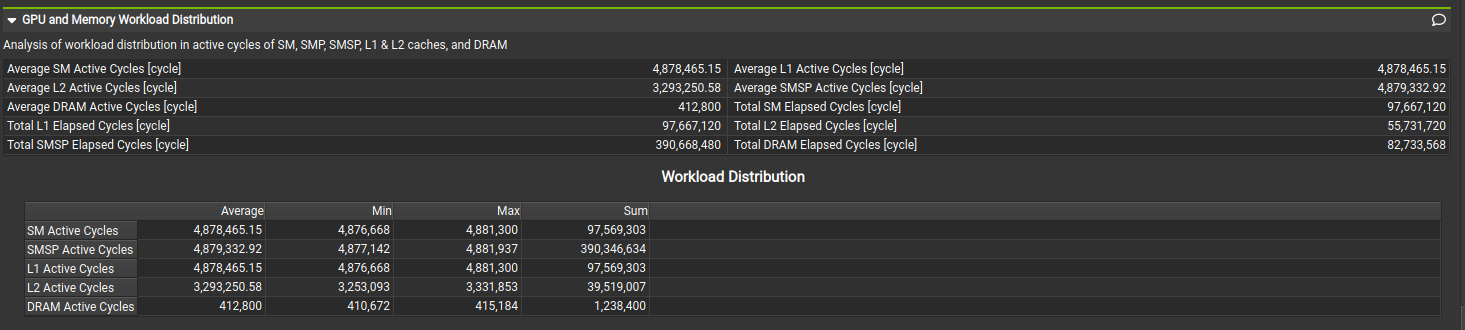
\includegraphics[width=0.95\linewidth]{figures/WorkloadDistribution.png}
    \caption{GPU and Memory Workload Distribution across Active Cycles}
    \label{fig:workload-distribution}
\end{figure}

\begin{figure}[H]
    \centering
    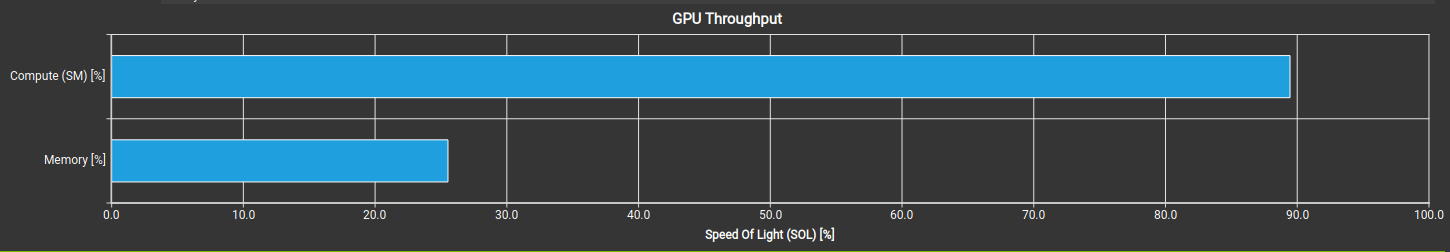
\includegraphics[width=0.9\linewidth]{figures/GPU_Throughput.png}
    \caption{Compute vs Memory Throughput as Percentage of Speed-of-Light}
    \label{fig:gpu-throughput}
\end{figure}

\textbf{Warp Behavior and Execution Bottlenecks.}

Figure~\ref{fig:warp-states} presents the breakdown of warp stalls. The most dominant stall reason was \textit{Tex Throttle}, followed by \textit{Short Scoreboard}, both indicative of memory-related latency.  
Figure~\ref{fig:pipe-utilization} further shows that the FP64 pipeline is over-utilized (89.5\% active cycles), potentially introducing bottlenecks.

\begin{figure}[H]
    \centering
    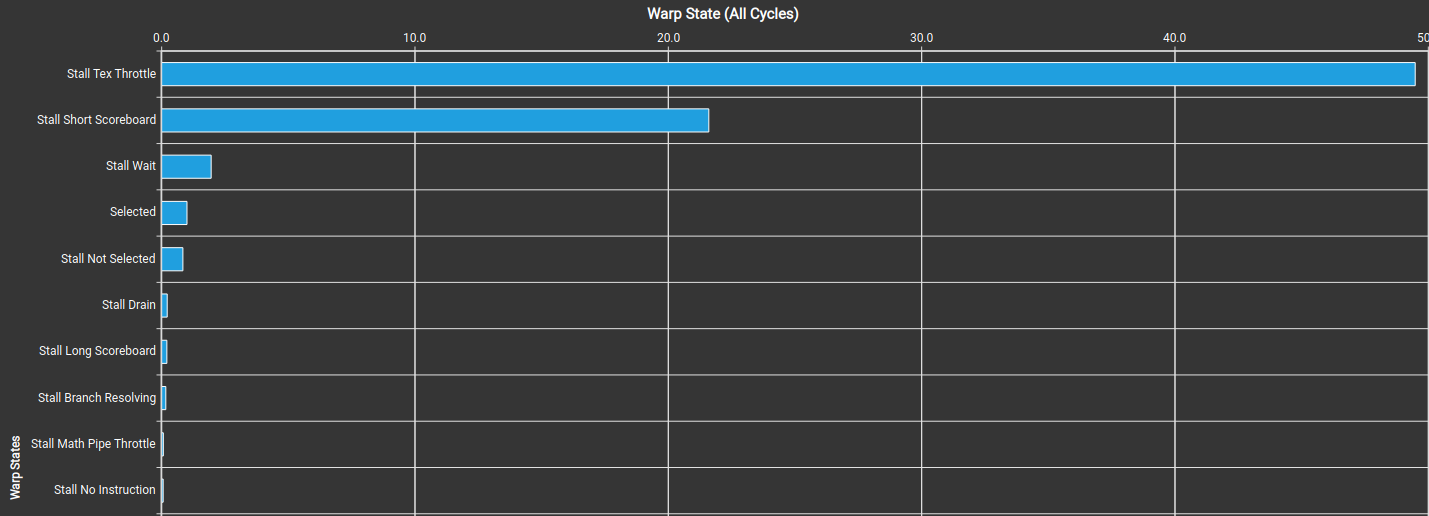
\includegraphics[width=0.95\linewidth]{figures/WarpState.png}
    \caption{Warp State Distribution during Kernel Execution}
    \label{fig:warp-states}
\end{figure}

\begin{figure}[H]
    \centering
    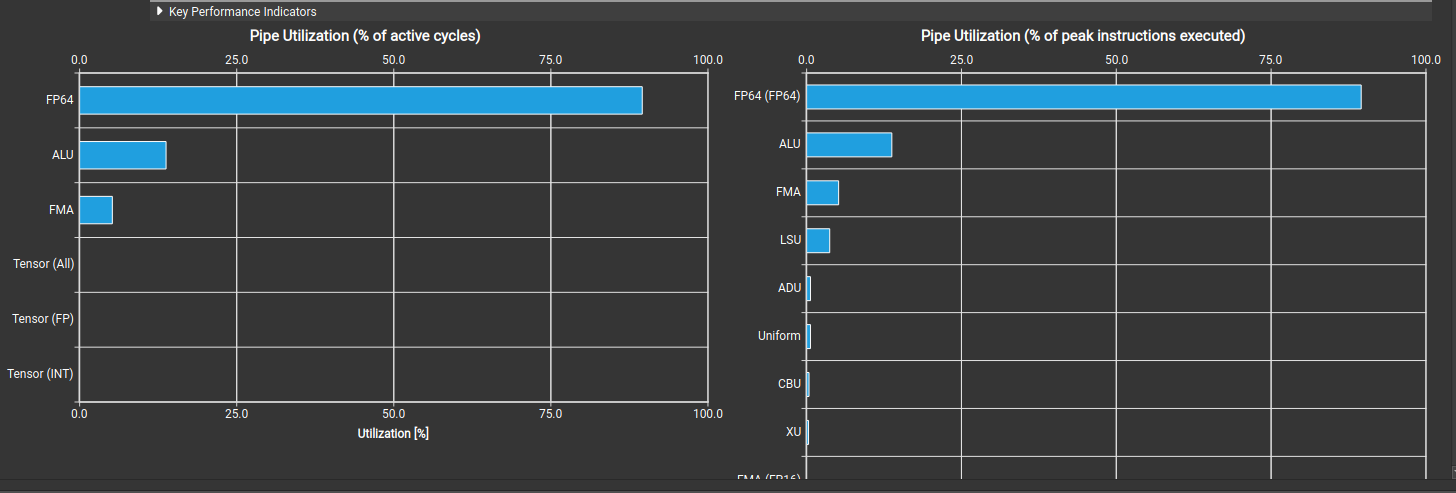
\includegraphics[width=0.95\linewidth]{figures/PipeUtilization.png}
    \caption{Pipe Utilization: FP64 Dominance and ALU/FMA Usage}
    \label{fig:pipe-utilization}
\end{figure}

\textbf{Memory Access and Cache Efficiency.}

Memory flow visualization in Figure~\ref{fig:memory-chart} shows strong L1/L2 cache performance with hit rates of 96\% and 98\% respectively.  
Figure~\ref{fig:l2-excess} shows that 94\% of L2 requests are uncoalesced, indicating room for improving memory access patterns via coalescing.

\begin{figure}[H]
    \centering
    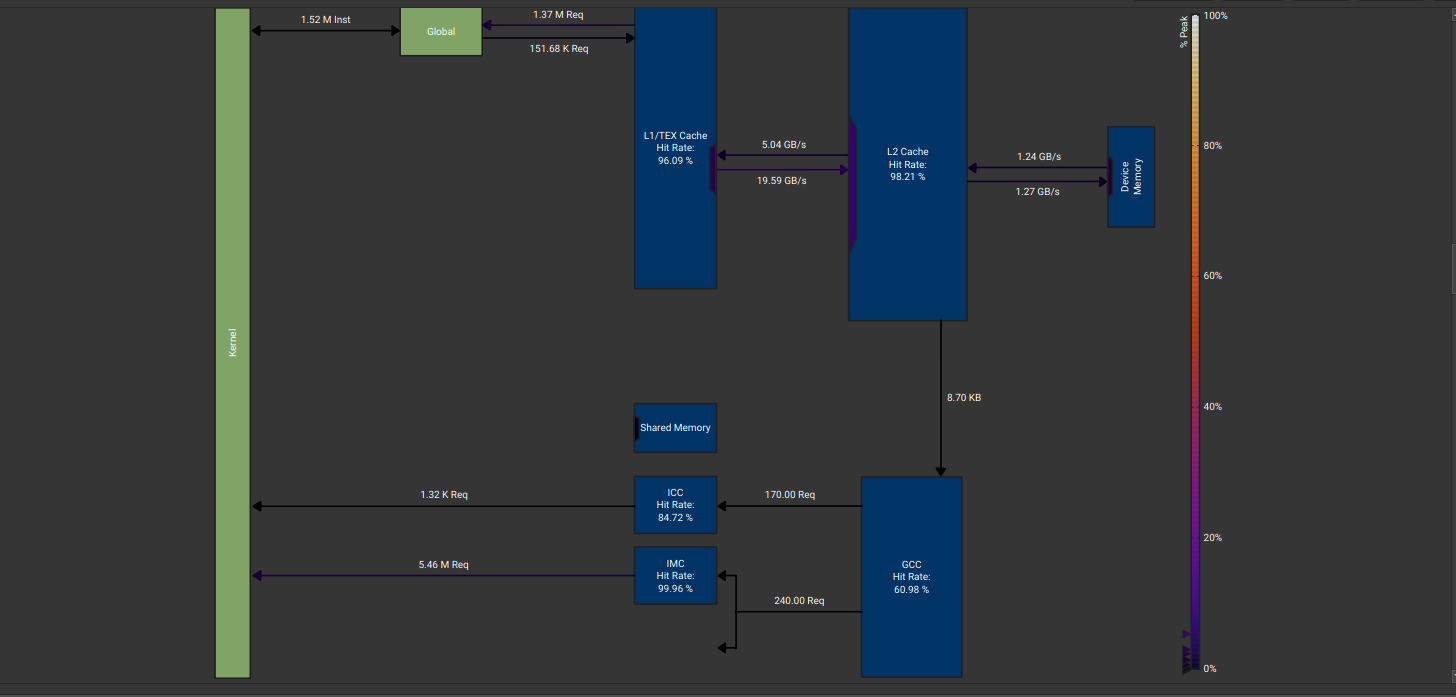
\includegraphics[width=0.9\linewidth]{figures/MemoryChart.png}
    \caption{Memory Access Pattern and Cache Hit Rates}
    \label{fig:memory-chart}
\end{figure}

\begin{figure}[H]
    \centering
    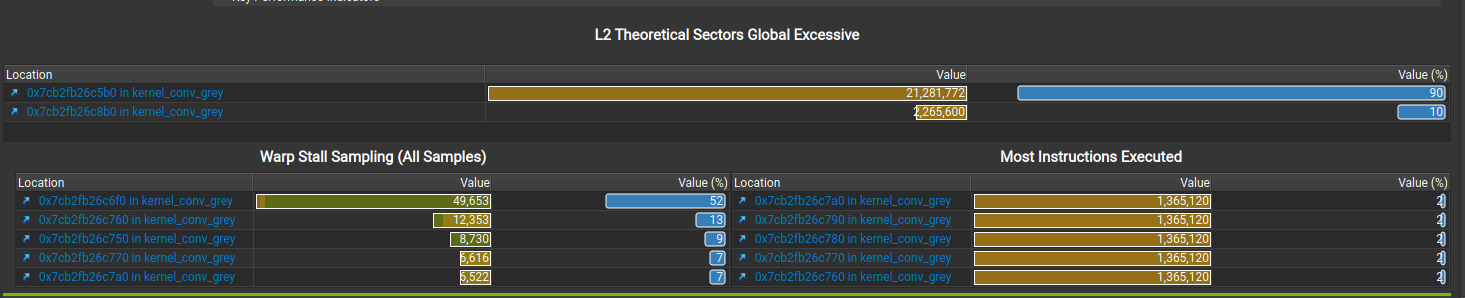
\includegraphics[width=0.9\linewidth]{figures/L2.png}
    \caption{L2 Cache: Global Access Sector Overuse and Warp Stalls}
    \label{fig:l2-excess}
\end{figure}

\textbf{Occupancy and Shared Memory Optimization.}

Nsight’s occupancy graphs (Figures~\ref{fig:occupancy-shared} and \ref{fig:occupancy-block}) show that using fewer registers and shared memory per block improves occupancy. The configuration around 256 threads per block with modest shared memory usage achieves optimal utilization.

\begin{figure}[H]
    \centering
    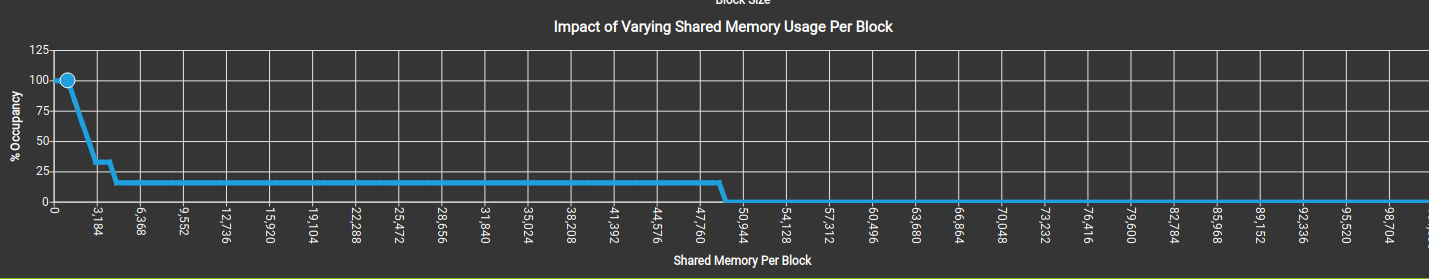
\includegraphics[width=0.9\linewidth]{figures/ImpactOfVarying_2.png}
    \caption{Occupancy vs Shared Memory Usage per Block}
    \label{fig:occupancy-shared}
\end{figure}

\begin{figure}[H]
    \centering
    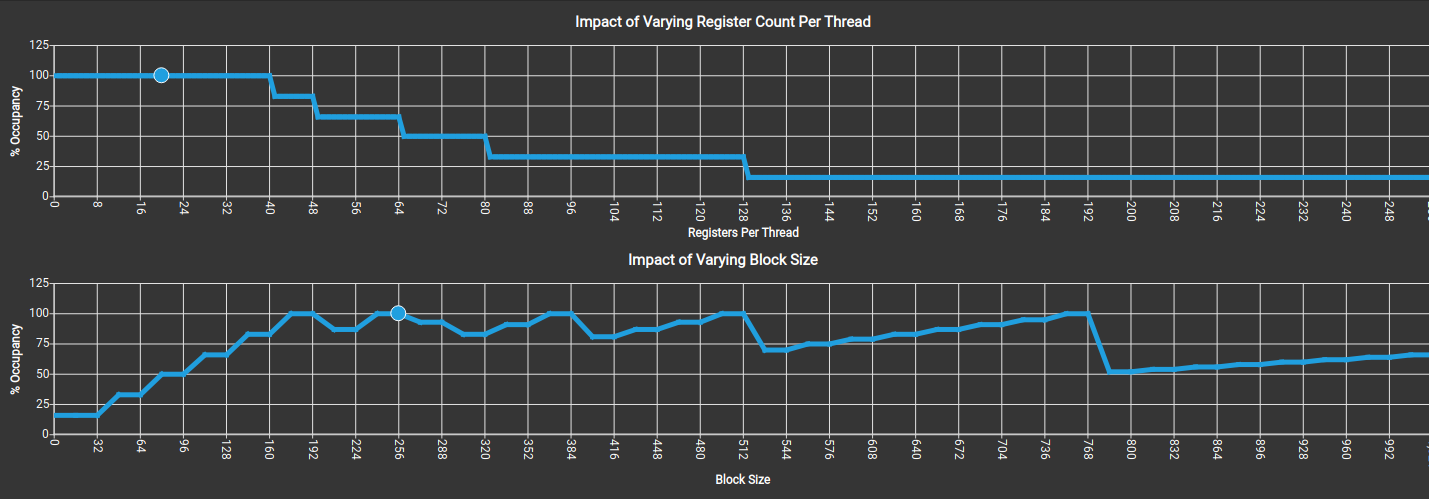
\includegraphics[width=0.9\linewidth]{figures/ImpactOfVarying.png}
    \caption{Occupancy vs Block Size and Register Usage}
    \label{fig:occupancy-block}
\end{figure}

\textbf{Performance Summary.}

The CUDA kernel demonstrated a speedup of over 11$\times$ compared to the sequential CPU implementation:

\[
\text{Speedup} = \frac{3100\text{ ms}}{265\text{ ms}} \approx 11.7\times
\]

\begin{table}[H]
    \centering
    \caption{Performance Comparison: CPU vs CUDA}
    \label{tab:speedup-table}
    \begin{tabular}{@{}lccc@{}}
        \toprule
        \textbf{Configuration} & \textbf{CPU Time (ms)} & \textbf{CUDA Time (ms)} & \textbf{Speedup} \\
        \midrule
        1920$\times$2520 Image & 3100 & 265 & 11.7$\times$ \\
        \bottomrule
    \end{tabular}
\end{table}

Overall, CUDA and Nsight Compute provided rich diagnostics, and the profiling insights suggest future directions for optimizing memory access patterns, reducing warp stalls, and increasing scheduler issue efficiency.





\subsection{\textbf{Multi-Core CPU}}

\subsubsection{\textbf{Weak Scaling}}

\textbf{A. Weak Scaling Analysis}
Weak scaling maintained constant workload per processing unit by proportionally increasing image size with N threads/processes for MPI-only (mpi\_conv) and hybrid OpenMP+MPI (parallelized) versions \cite{Gustafson1988}.

\textbf{1. Aggregate Weak Scaling Performance Metrics (Fig.~\ref{fig:weak-scaling-metrics})}
\begin{figure}[H]
    \centering
    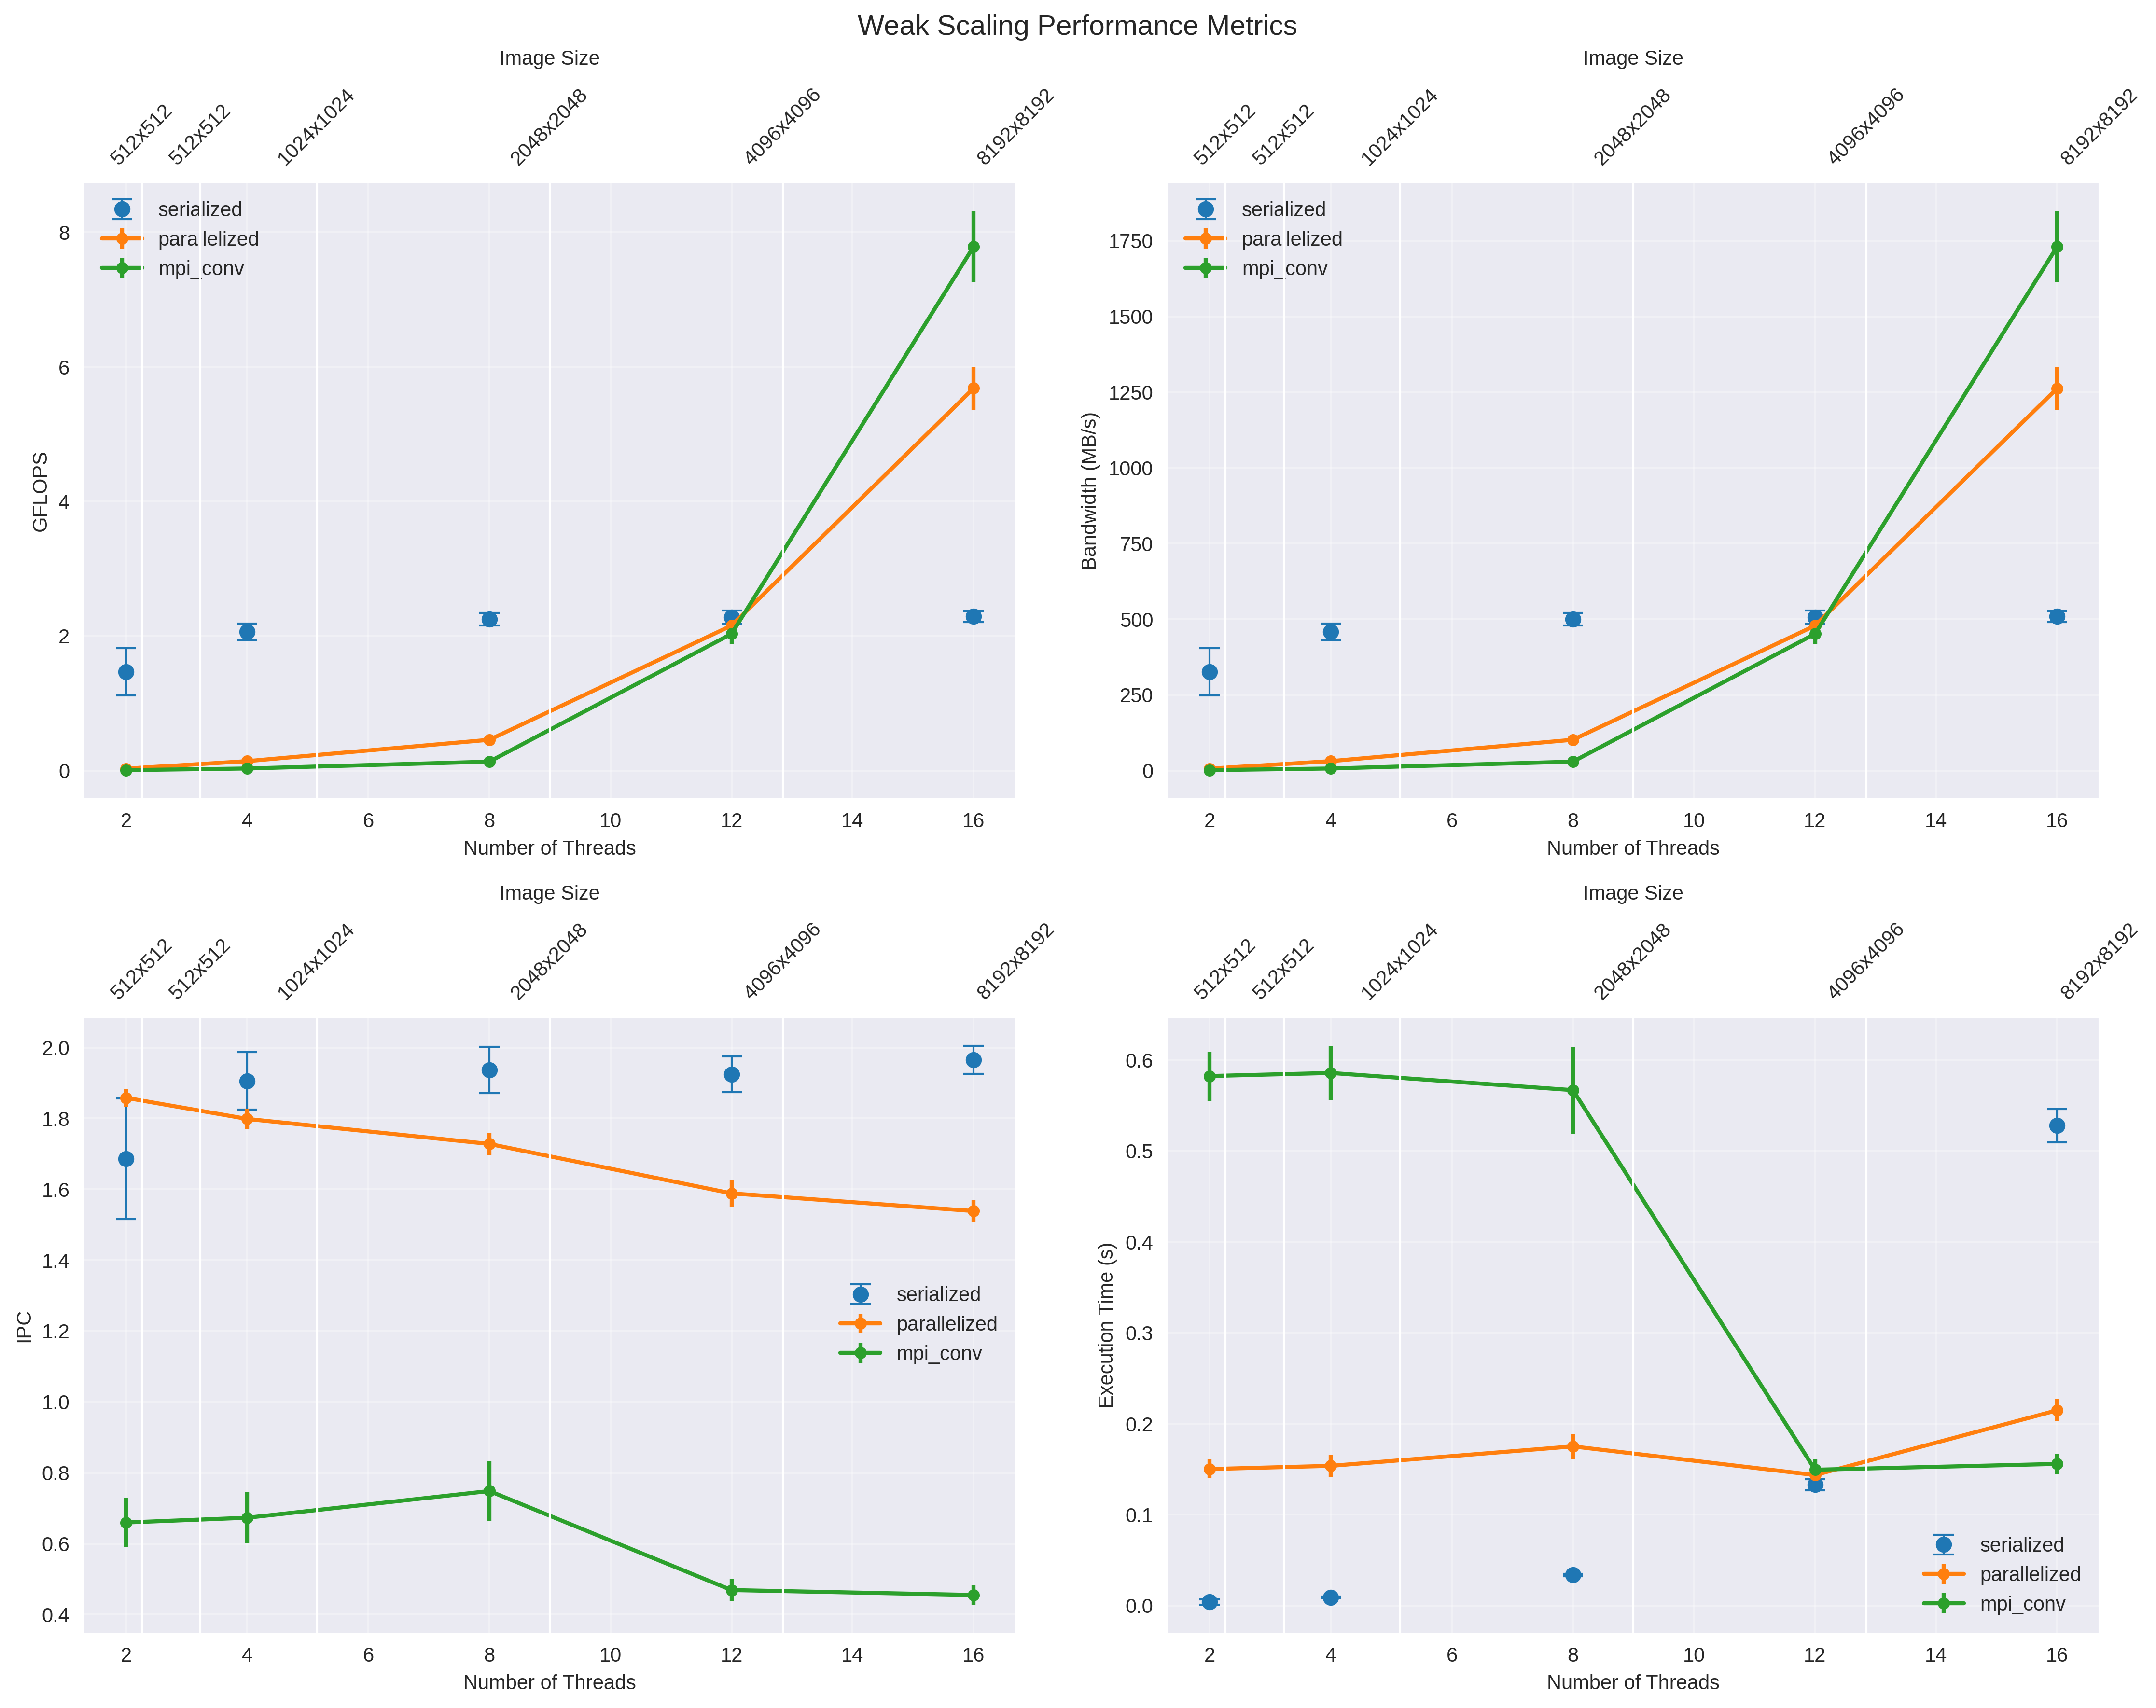
\includegraphics[width=0.9\linewidth]{figures/weak_scaling_metrics.png}
    \caption{Weak Scaling Metrics: GFLOPS, Memory Bandwidth, IPC, Execution Time vs. threads.}
    \label{fig:weak-scaling-metrics}
\end{figure}
    \textbf{GFLOPS:} Both parallel versions scaled GFLOPS upwards; `parallelized` consistently higher.
    \textbf{Memory Bandwidth:} Both increased usage; `parallelized` sustained higher bandwidth.
    \textbf{IPC:} `parallelized` maintained higher, stable IPC (~1.8-1.9); mpi\_conv lower (~0.6-0.7), dipping late.
    \textbf{Execution Time:} `parallelized` showed excellent weak scaling (near-constant time ~0.15-0.18s); mpi\_conv higher (~0.20-0.25s) with a slight upward trend.

\textbf{2. Detailed Weak Scaling Analysis via 3D Surface Plots}
    \textbf{Memory Bandwidth (Fig.~\ref{fig:weak-scaling-bandwidth-3d}):} `parallelized` surface consistently higher, indicating superior bandwidth utilization.
\begin{figure}[H]
    \centering
    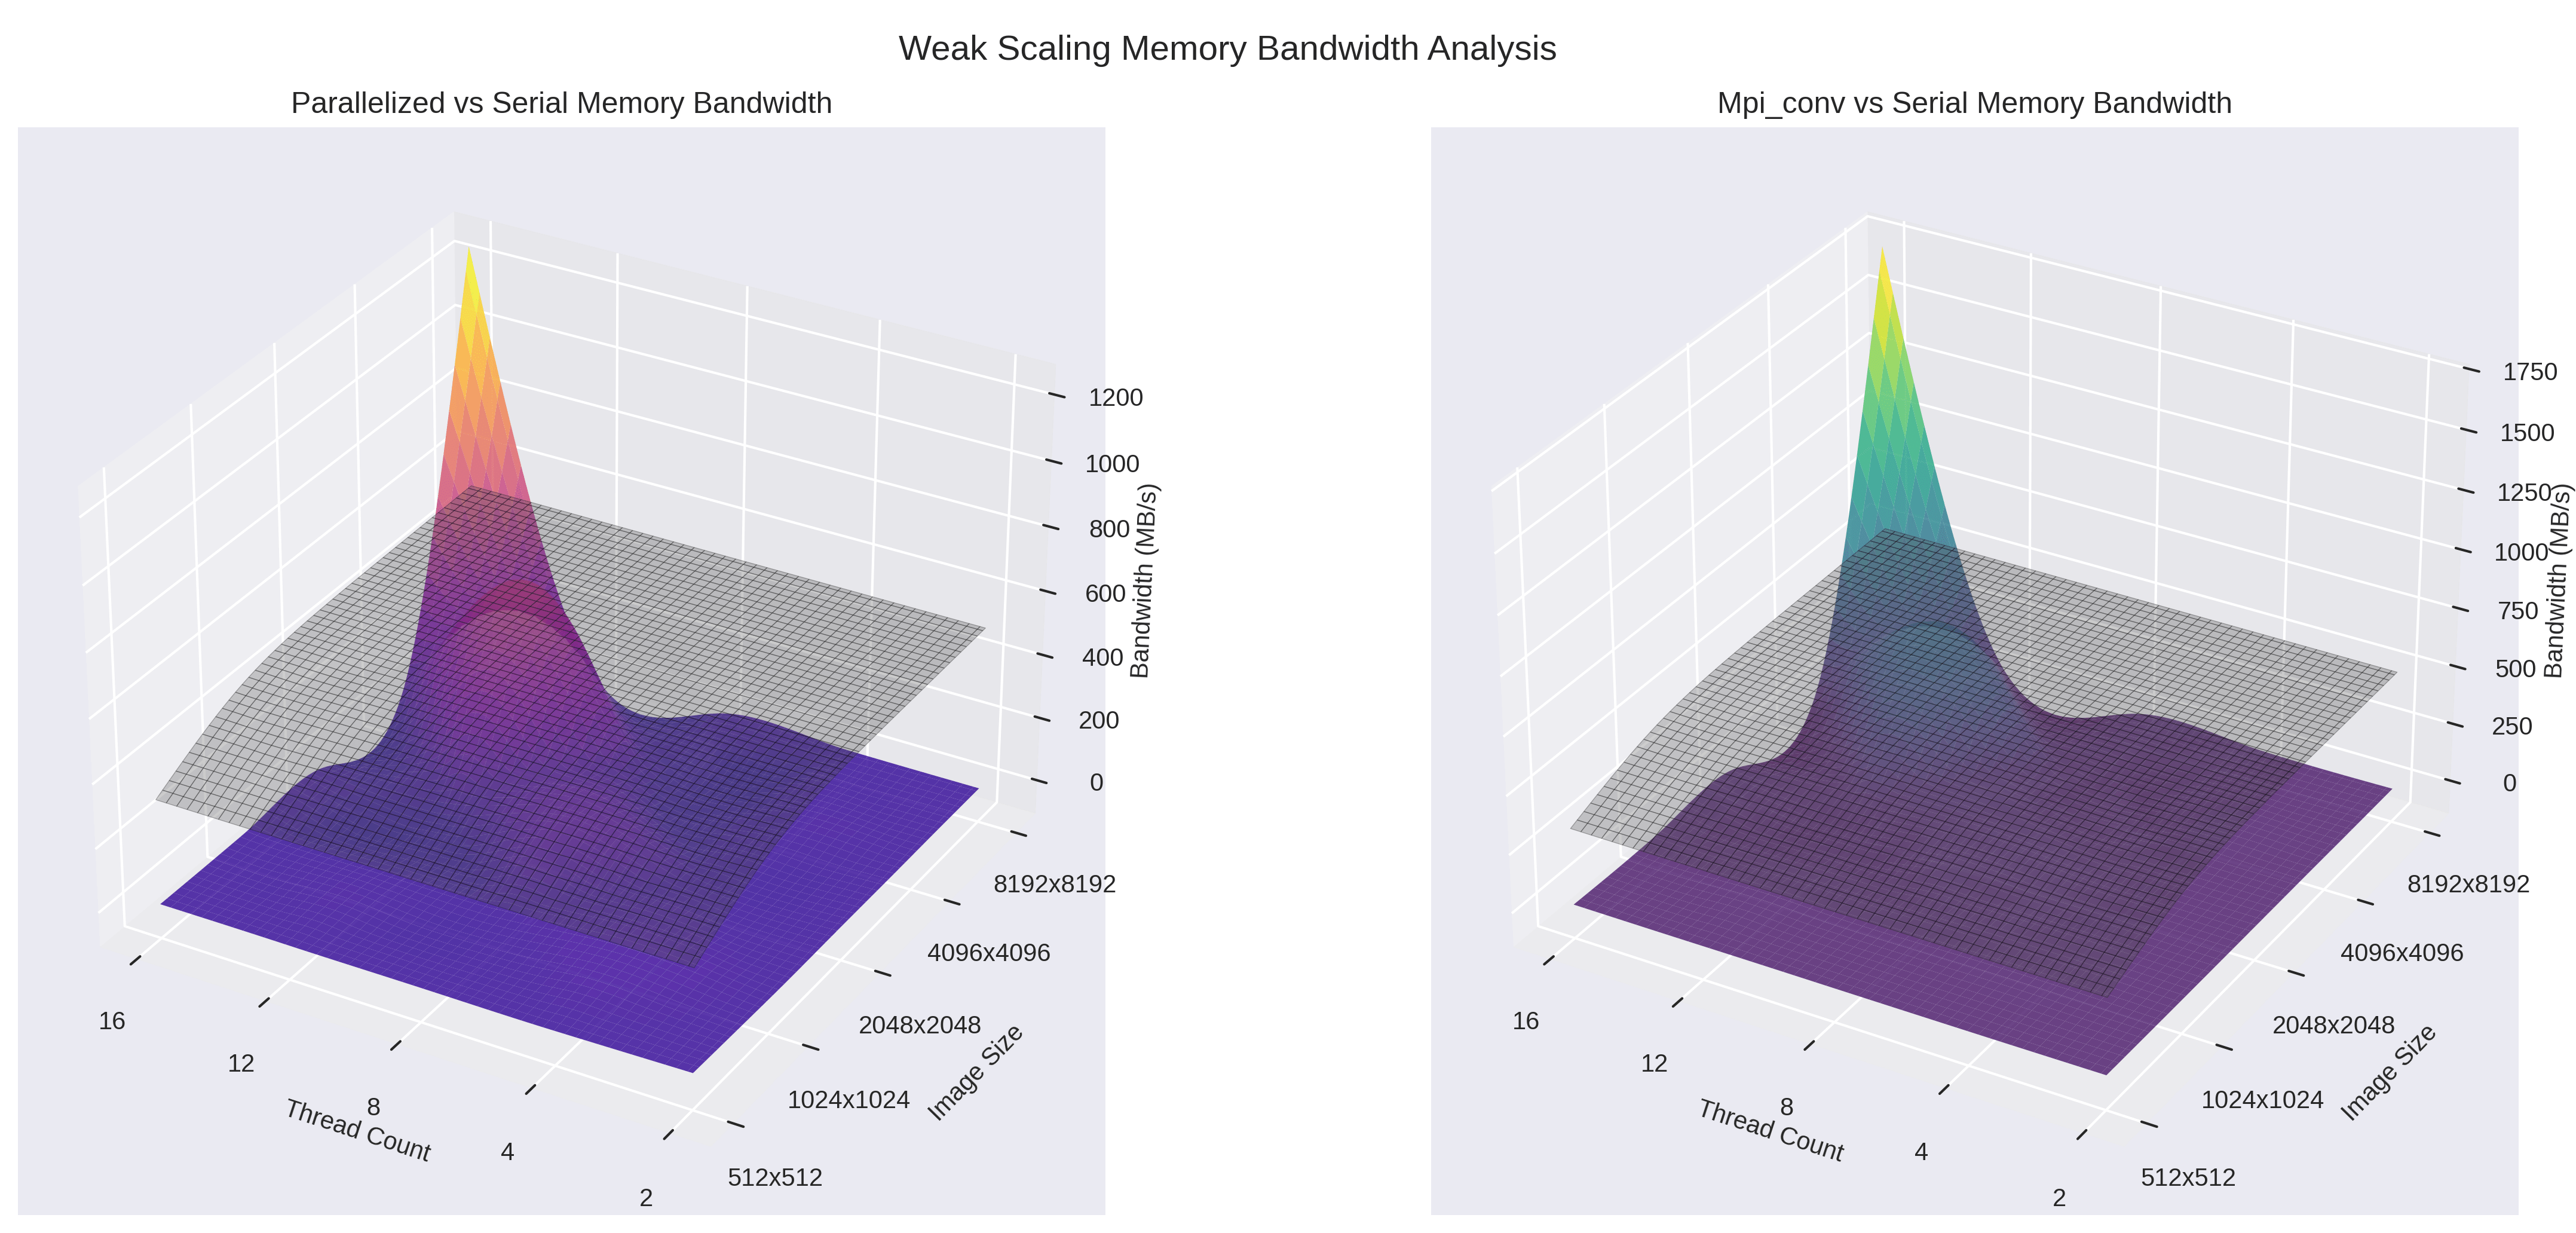
\includegraphics[width=0.9\linewidth]{figures/bandwidth_3d_surfaces.png}
    \caption{Weak Scaling Memory Bandwidth (3D): `parallelized` (L) & mpi\_conv (R) vs. Serial.}
    \label{fig:weak-scaling-bandwidth-3d}
\end{figure}
    \textbf{L1 Cache Miss Rate (Fig.~\ref{fig:weak-scaling-l1-miss-3d}):} `parallelized` exhibited low, flat L1 miss rates; mpi\_conv showed peaks, suggesting poorer L1 locality \cite{Yoon2012}.
\begin{figure}[H]
    \centering
    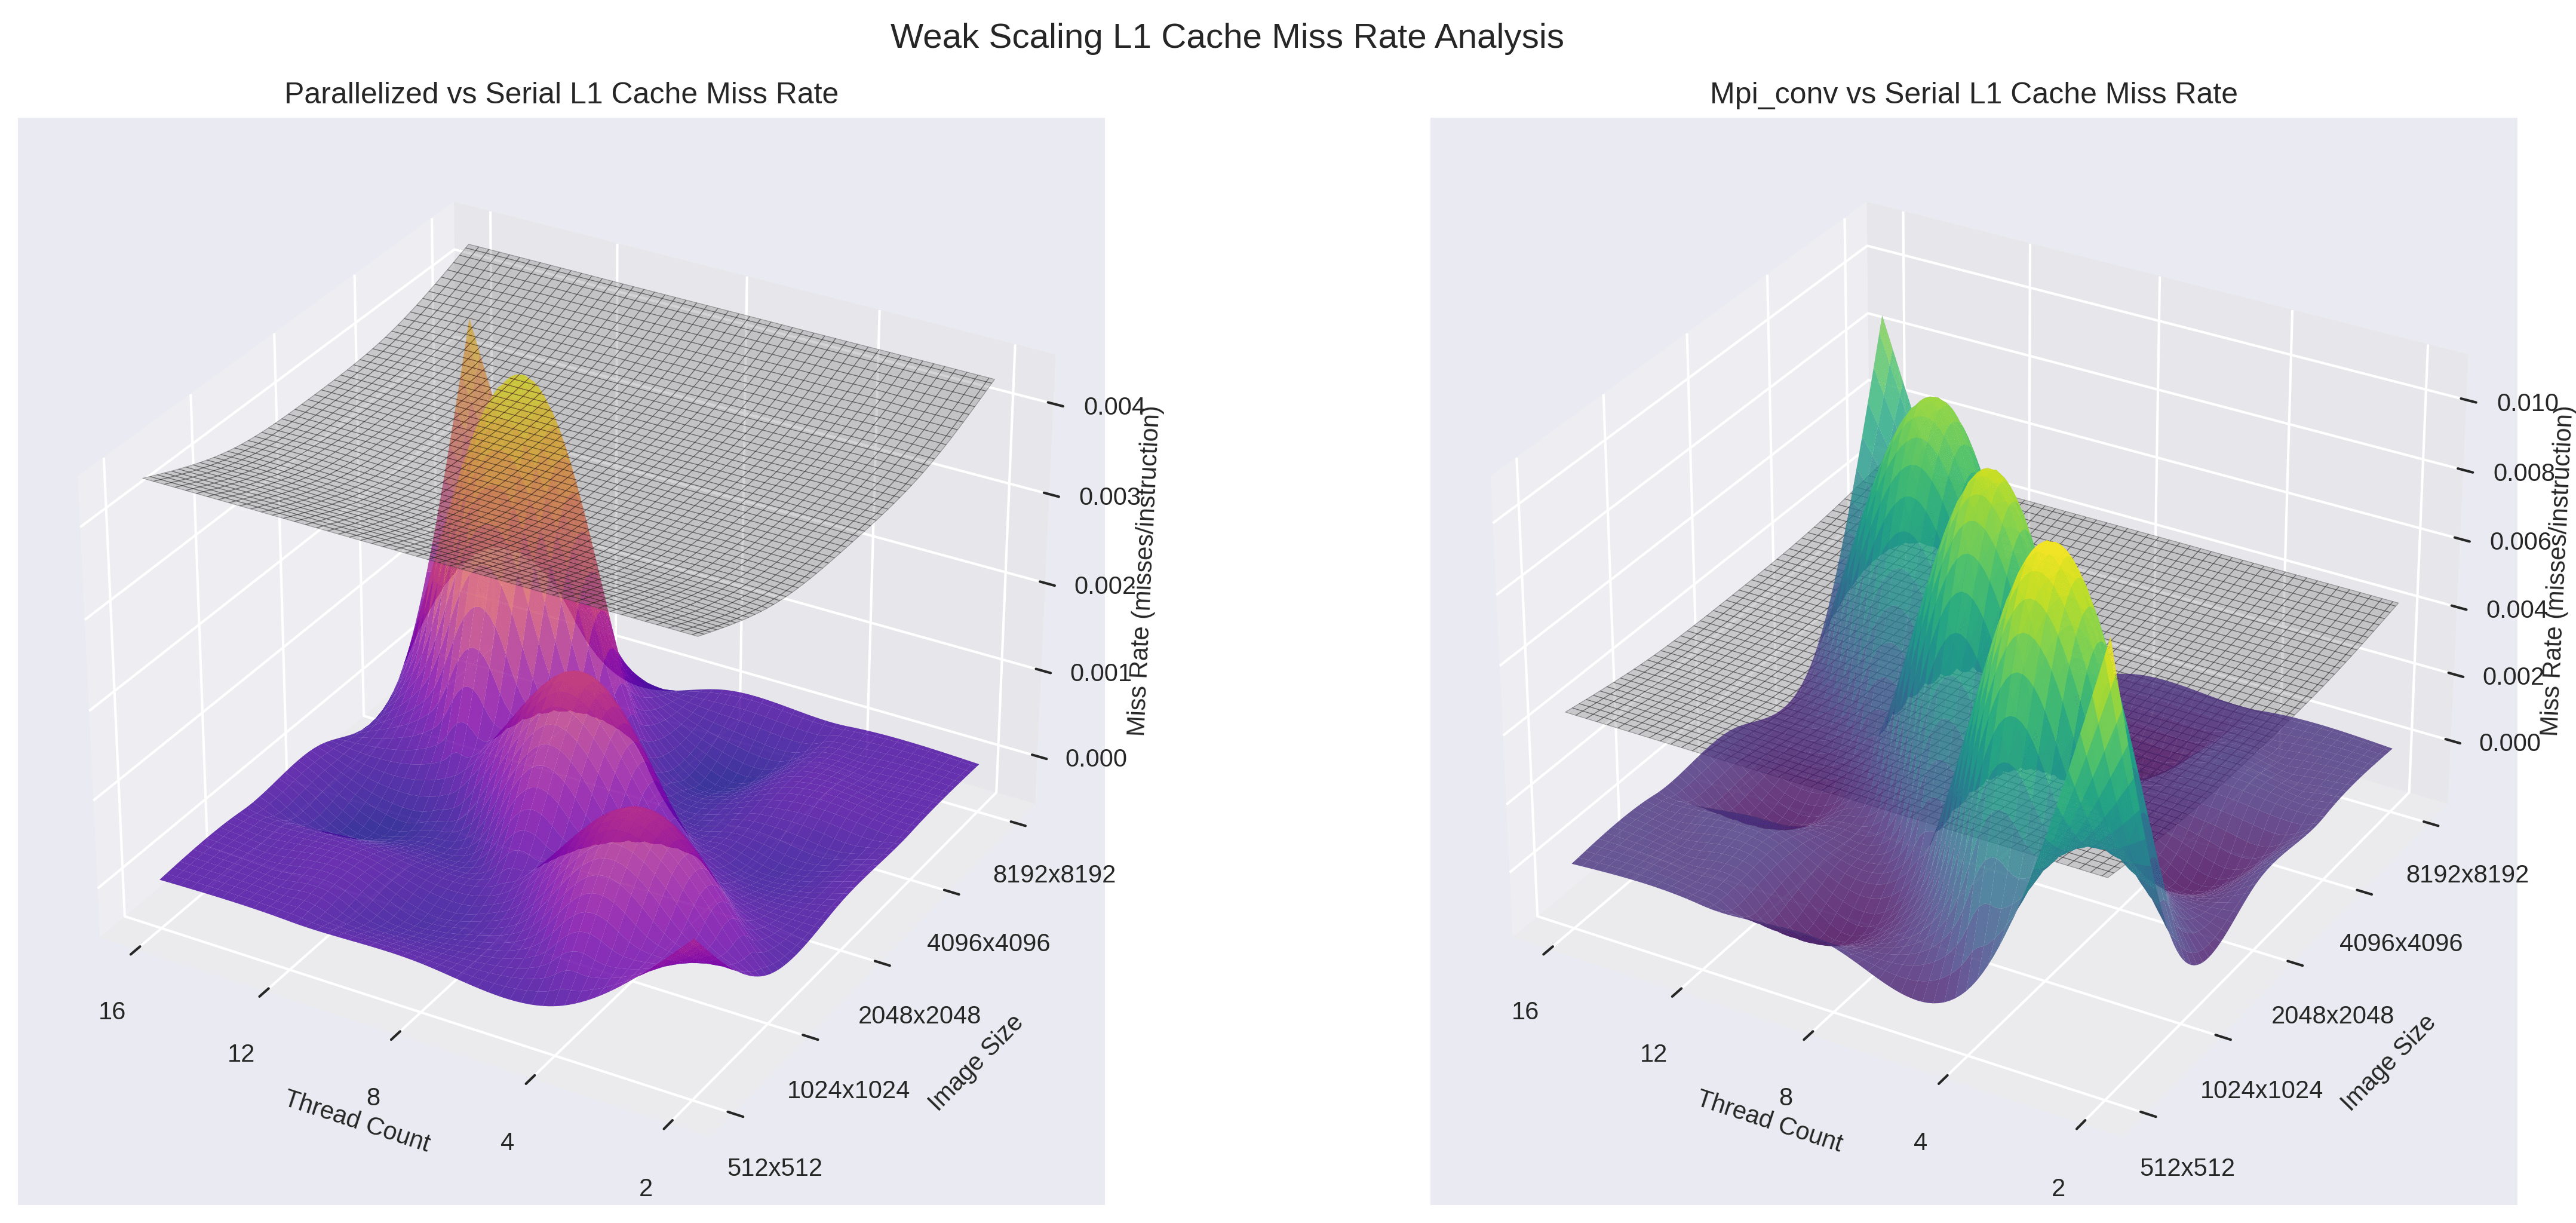
\includegraphics[width=0.9\linewidth]{figures/l1_miss_rate_3d_surfaces.png}
    \caption{Weak Scaling L1 Cache Miss Rate (3D): `parallelized` (L) & mpi\_conv (R) vs. Serial.}
    \label{fig:weak-scaling-l1-miss-3d}
\end{figure}
    \textbf{GFLOPS/s (Fig.~\ref{fig:weak-scaling-gflops-3d}):} `parallelized` GFLOPS surface consistently higher and smoother.
\begin{figure}[H]
    \centering
    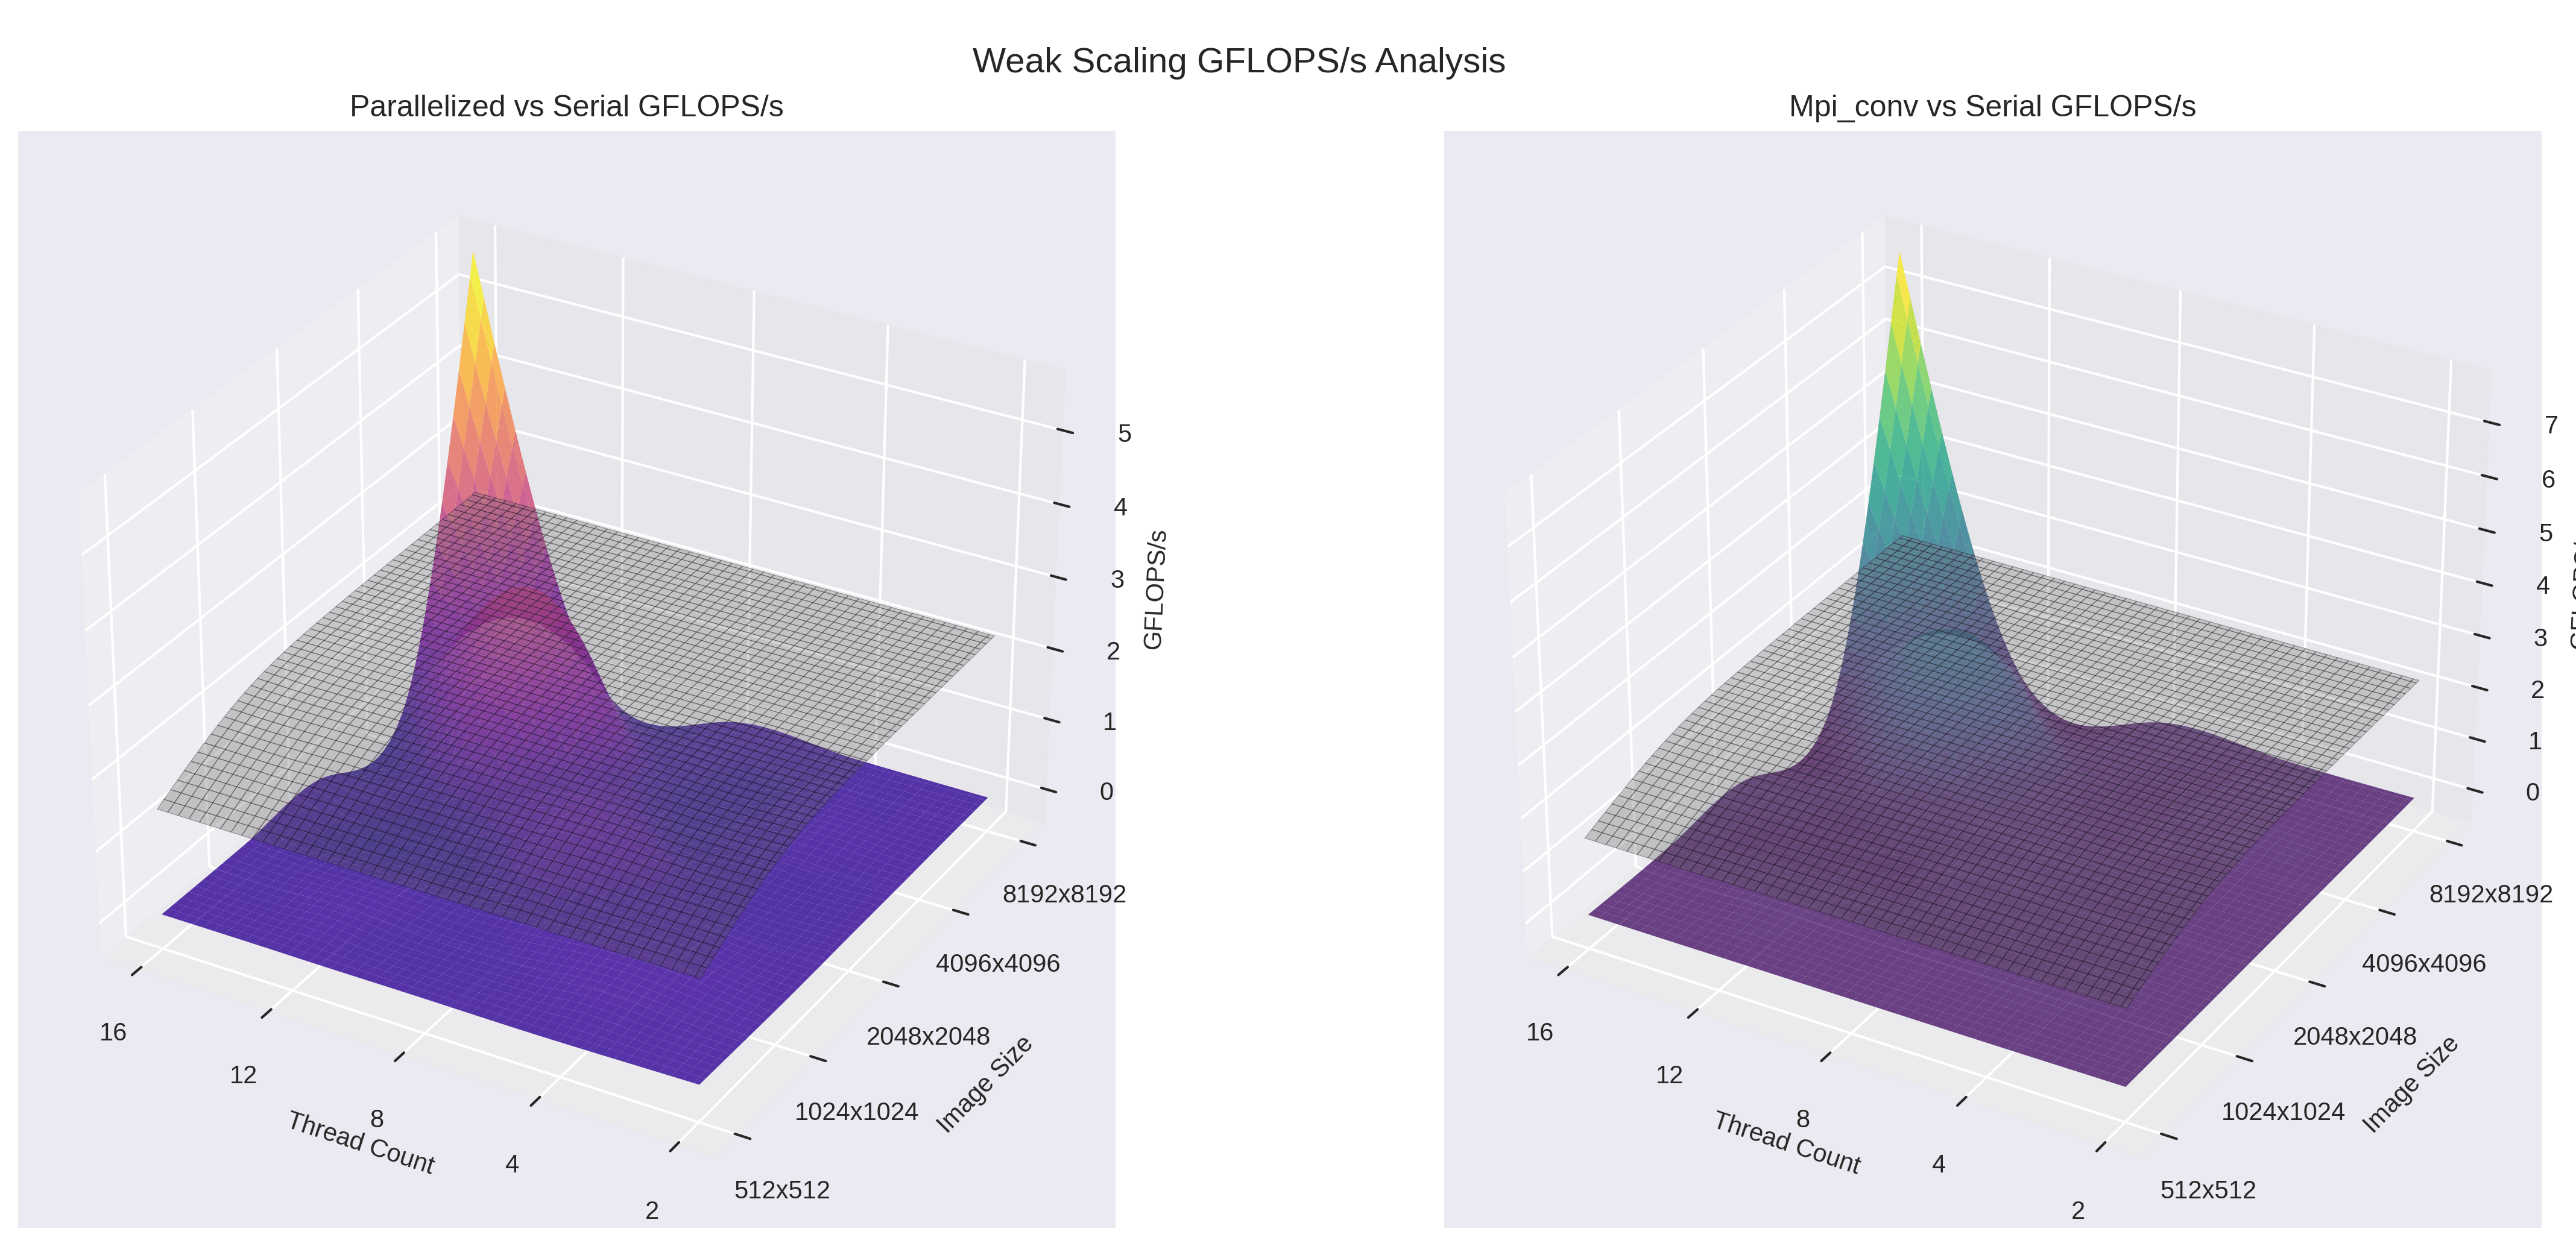
\includegraphics[width=0.9\linewidth]{figures/gflops_3d_surfaces.png}
    \caption{Weak Scaling GFLOPS/s (3D): `parallelized` (L) & mpi\_conv (R) vs. Serial.}
    \label{fig:weak-scaling-gflops-3d}
\end{figure}
    \textbf{Execution Time (Fig.~\ref{fig:weak-scaling-execution-time-3d}):} `parallelized` surface flatter and lower, confirming near-ideal weak scaling.
\begin{figure}[H]
    \centering
    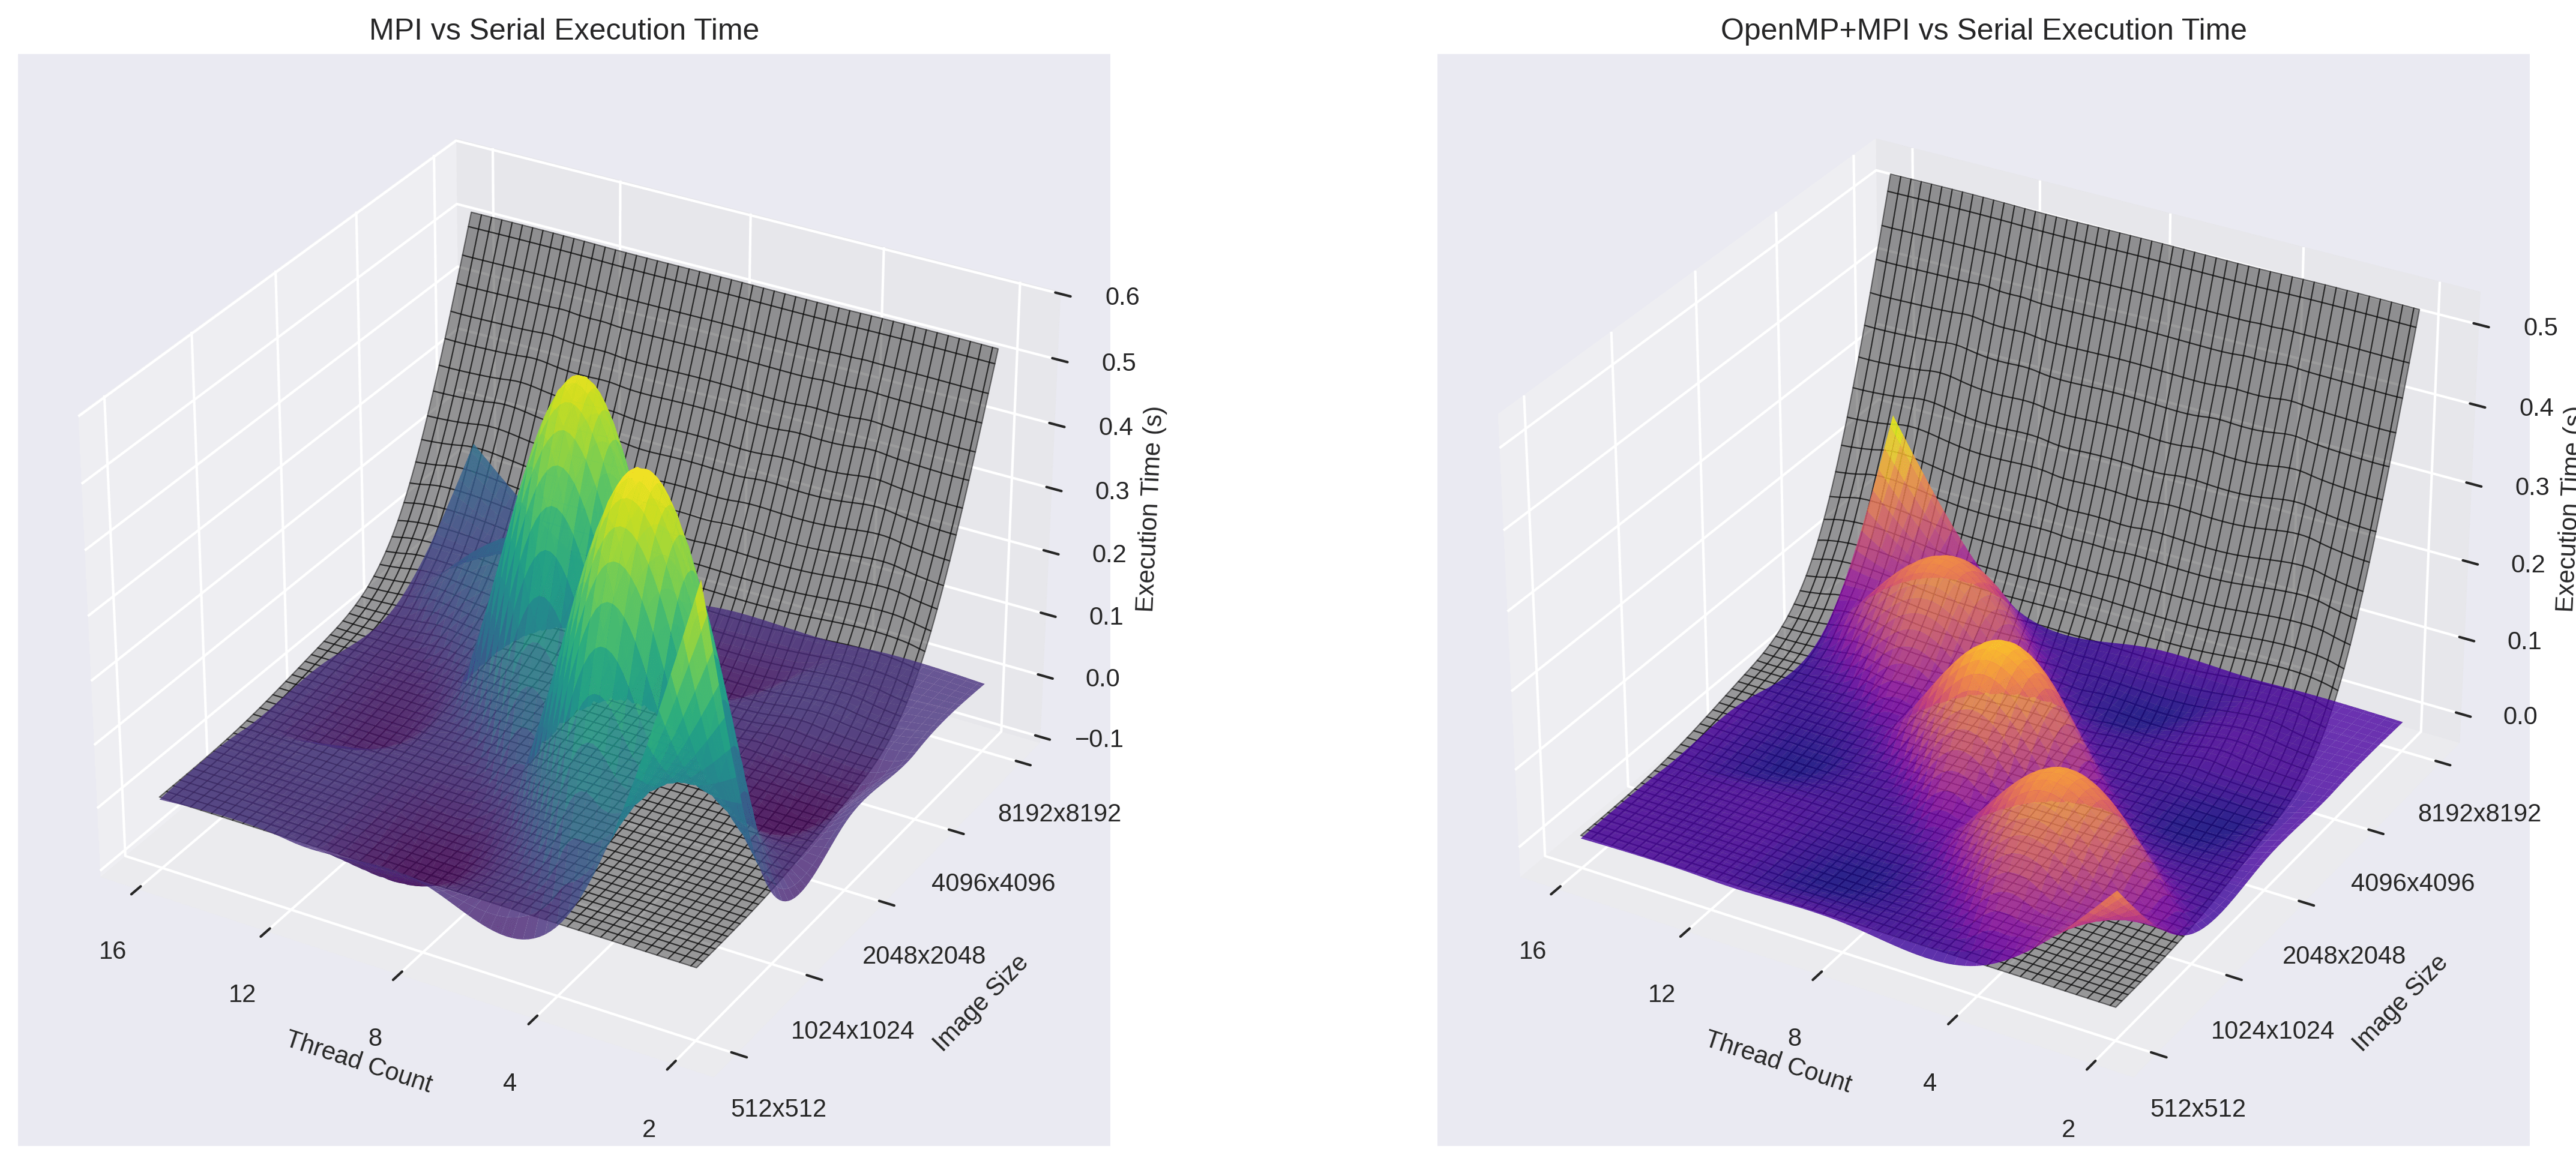
\includegraphics[width=0.9\linewidth]{figures/weak_scaling_3d_surfaces.png}
    \caption{Weak Scaling Execution Time (3D): mpi\_conv (L) & `parallelized` (R) vs. Serial.}
    \label{fig:weak-scaling-execution-time-3d}
\end{figure}

\textbf{3. Summary of Weak Scaling Findings}
\begin{itemize}
    \item Hybrid `parallelized` (OpenMP+MPI) outperformed MPI-only mpi\_conv, achieving near-ideal weak scaling with constant execution time.
    \item mpi\_conv, while scalable, showed lower efficiency, linked to higher L1 miss rates and MPI overheads.
    \item Hybrid's superiority likely due to lower OpenMP overheads for intra-node tasks, better shared-memory cache use, and finer load balancing \cite{Gawrych2023}.
\end{itemize}

\subsubsection{\textbf{Strong Scaling}}

Strong scaling used a fixed problem size (8192x8192 in this case) with increasing units (1-16), analyzed via Amdahl's Law \cite{hager2021hpc}.

\textbf{1. Speedup and Amdahl's Law (Fig.~\ref{fig:amdahls-law})}
\begin{figure}[H]
    \centering
    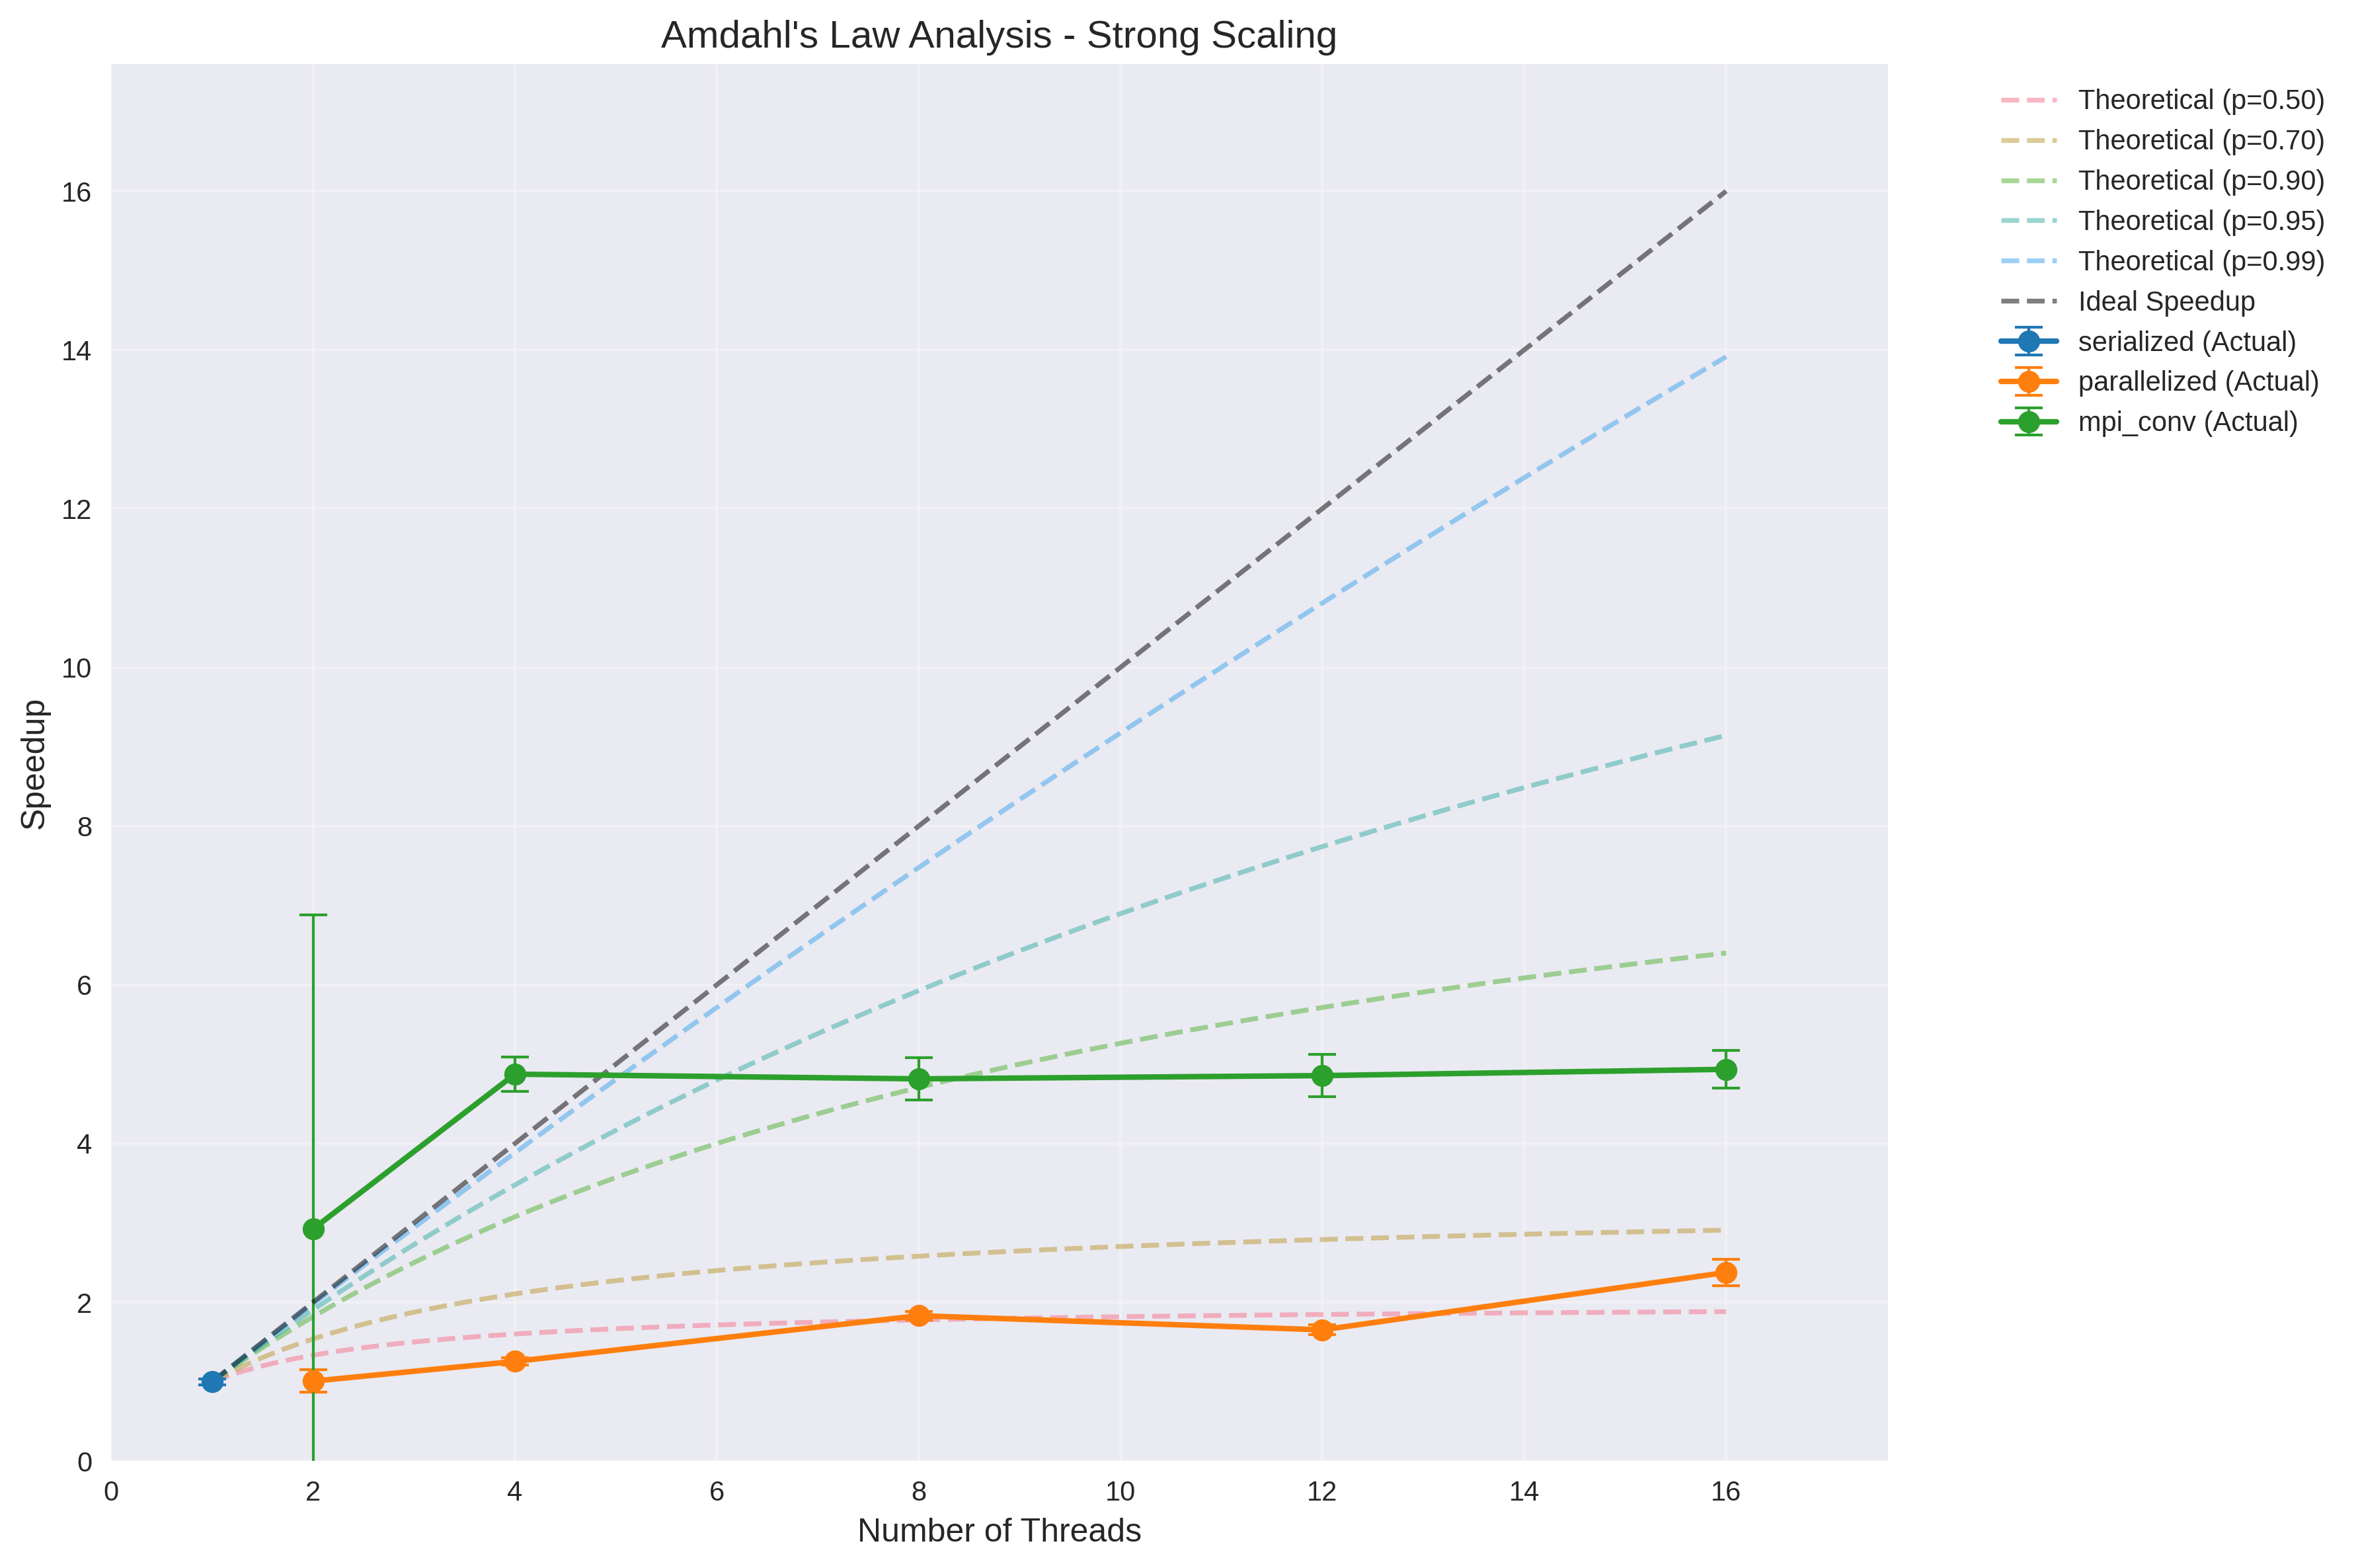
\includegraphics[width=0.7\linewidth]{figures/amdahls_law.png}
    \caption{Strong Scaling Speedup vs. Threads: mpi\_conv & `parallelized` vs. Amdahl's Law \cite{Rajput2013}.}
    \label{fig:amdahls-law}
\end{figure}
    \textbf{mpi\_conv:} Good initial speedup (peak ~4.9x at 4 threads), then plateaued, limited by sequential portions or MPI overheads.
    \textbf{`parallelized`:} Much lower speedup (max ~2.35x), significantly limited by overheads for the fixed problem size.
    \textbf{Comparison:} mpi\_conv scaled better initially; `parallelized` struggled with hybrid overheads.

\textbf{2. Strong Scaling Performance Metrics (Figs.~\ref{fig:strong-scaling-metrics-all}-\ref{fig:strong-scaling-l1-miss})}
\begin{figure}[H]
    \centering
    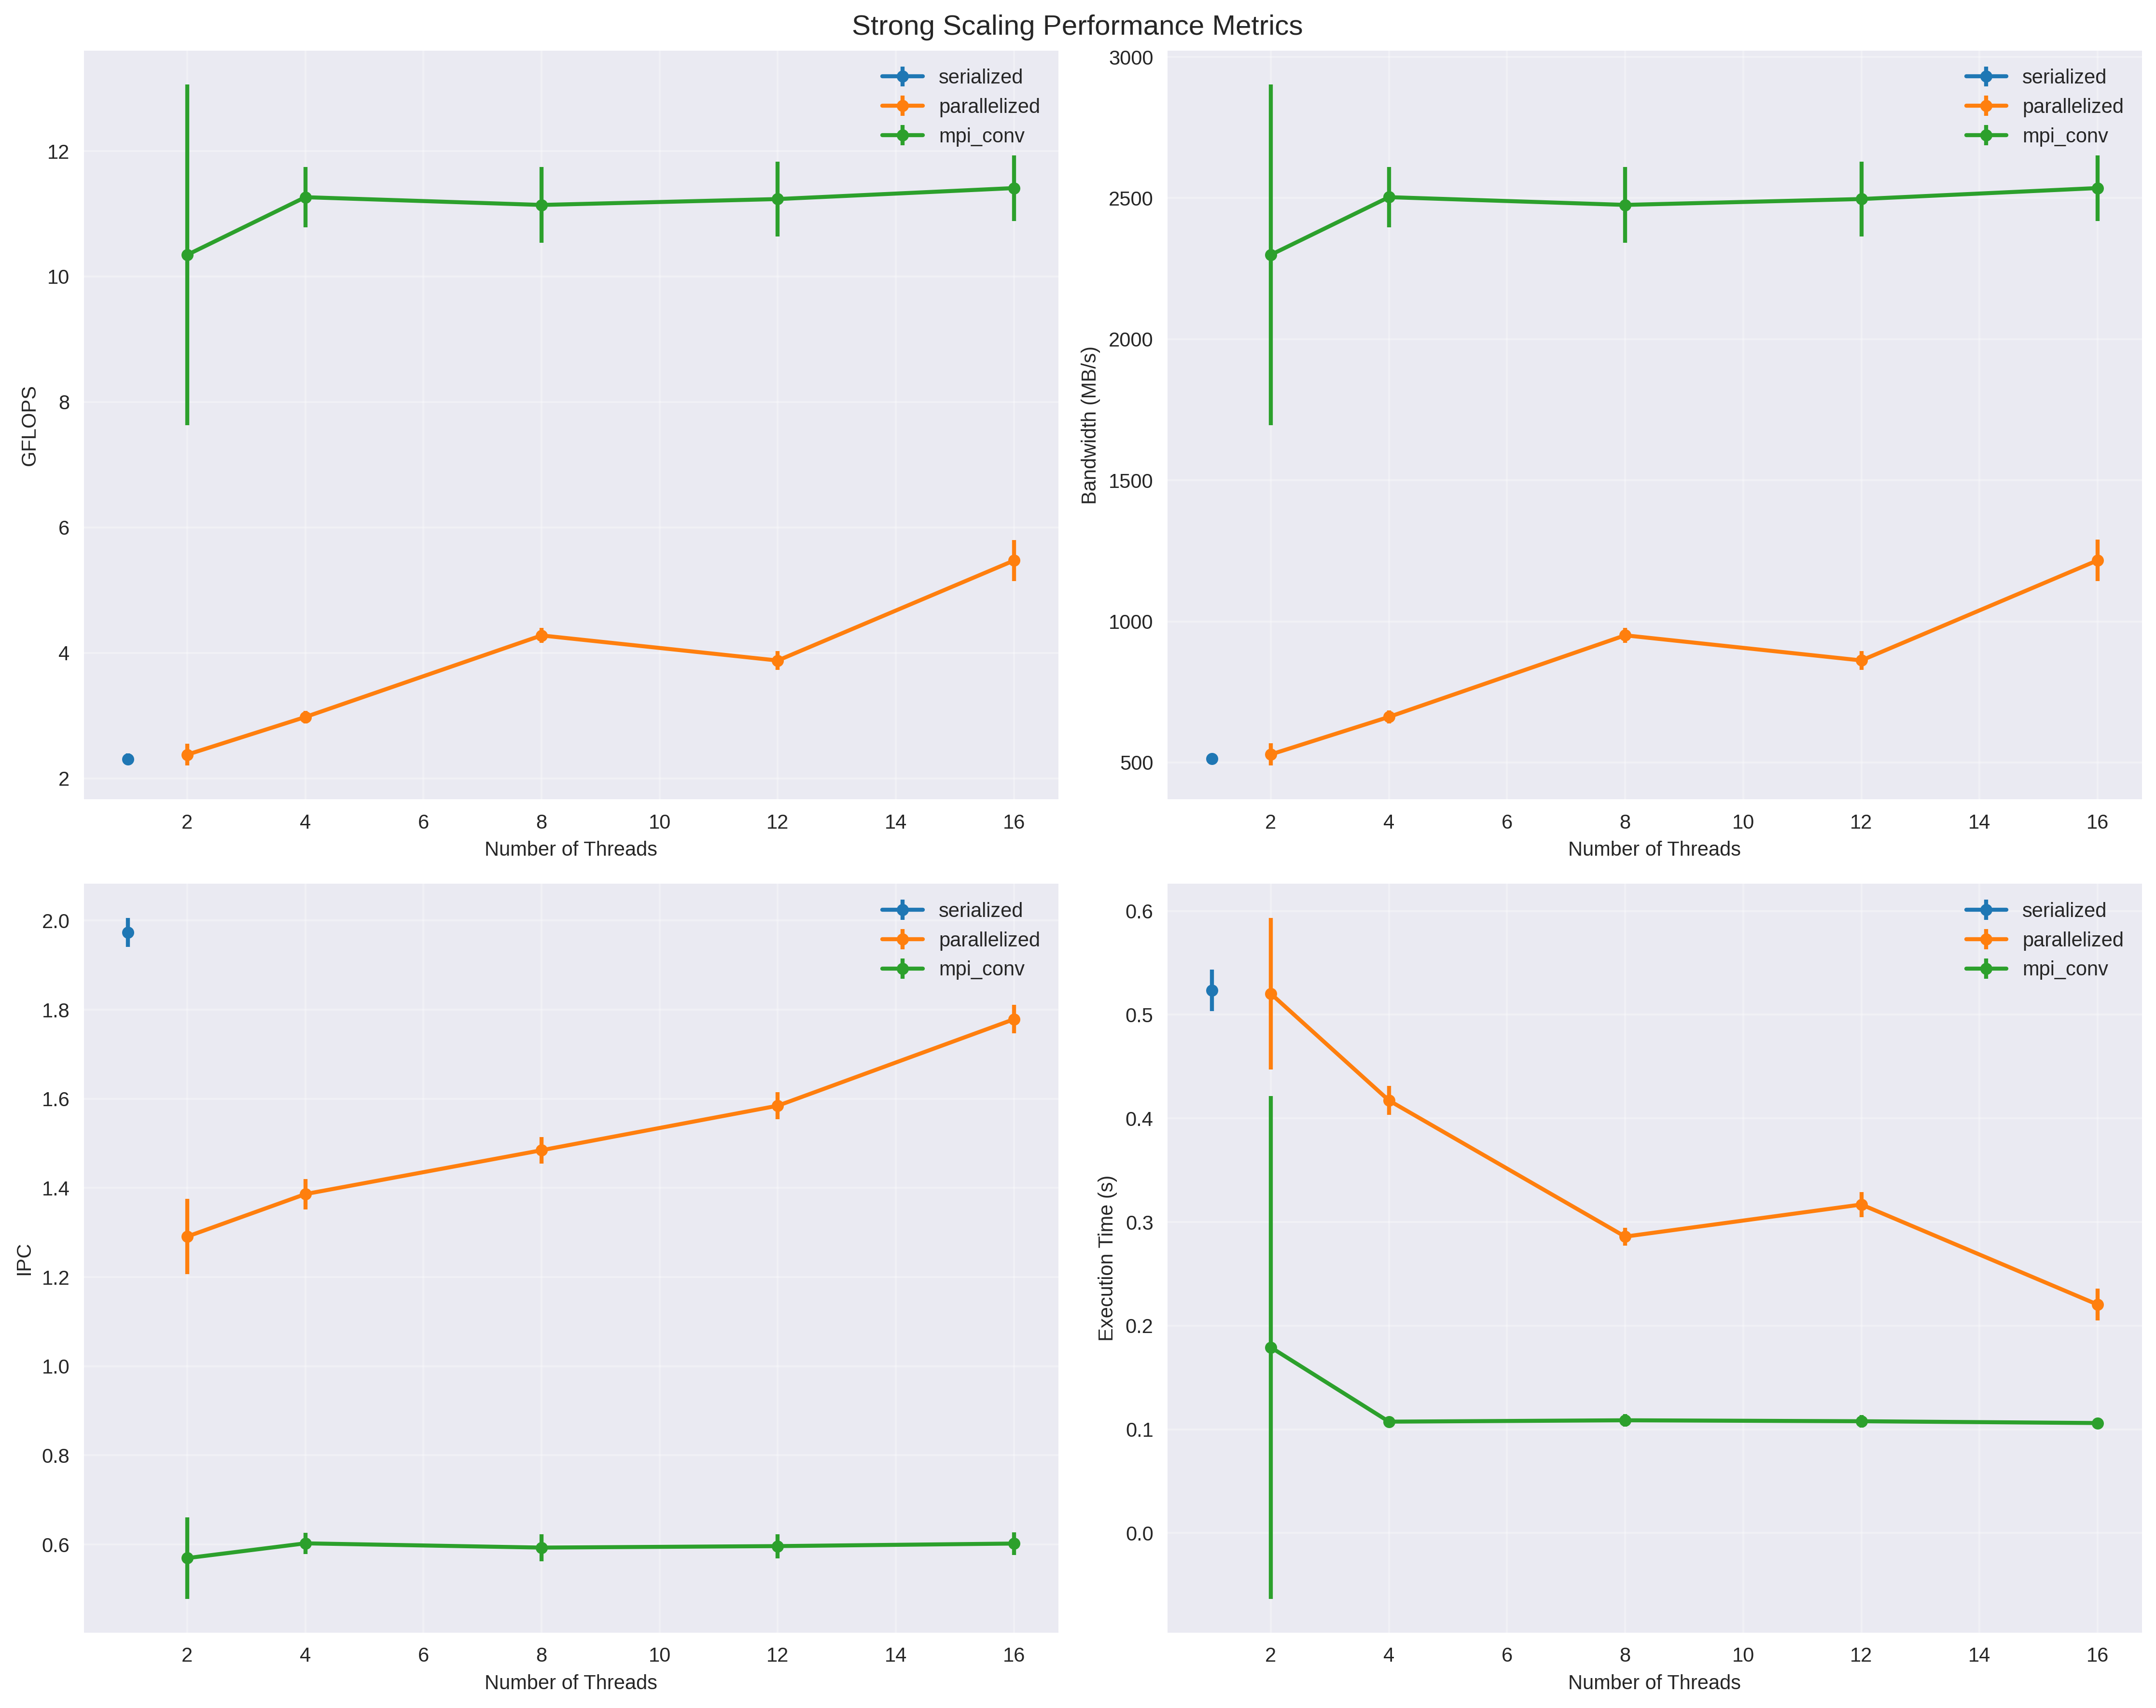
\includegraphics[width=0.9\linewidth]{figures/strong_scaling_metrics.png}
    \caption{Strong Scaling Metrics: GFLOPS, Bandwidth, IPC, Exec. Time vs. threads \cite{Wang2023}.}
    \label{fig:strong-scaling-metrics-all}
\end{figure}
    \textbf{GFLOPS (Fig.~\ref{fig:strong-scaling-gflops}):} mpi\_conv higher throughput, plateaued; `parallelized` consistently lower.
\begin{figure}[H] \centering 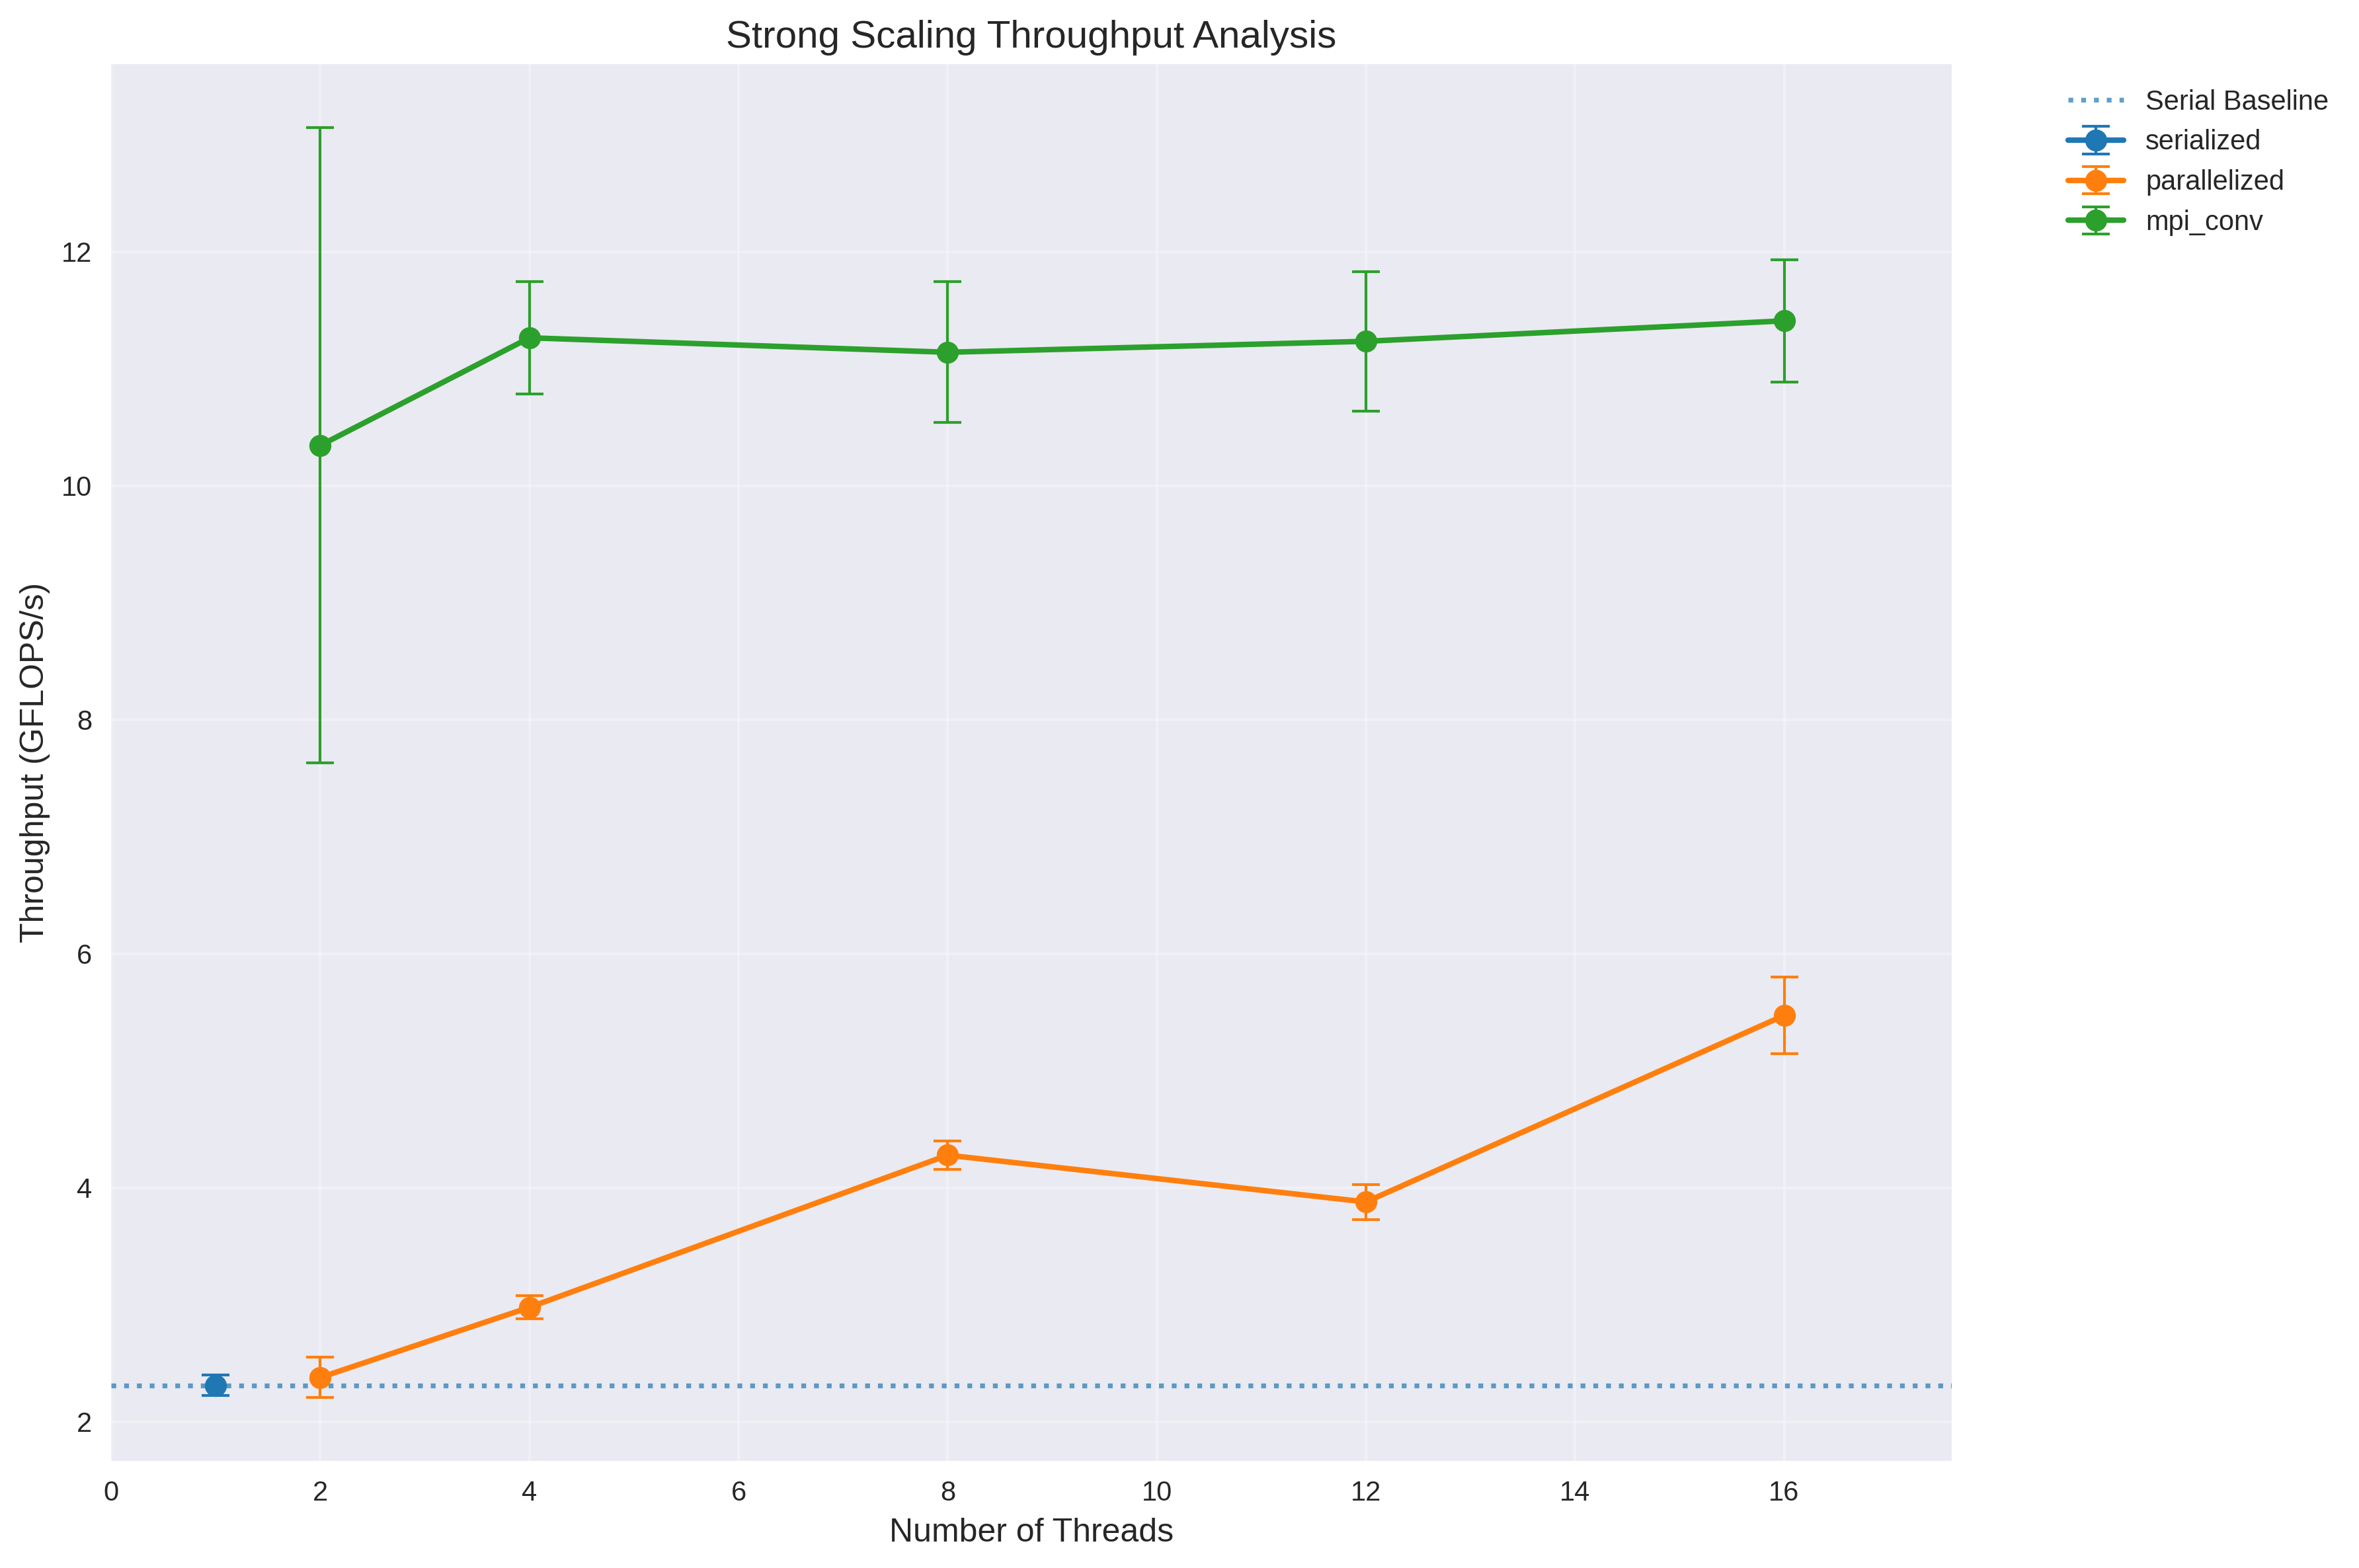
\includegraphics[width=0.7\linewidth]{figures/gflops_vs_threads.png} \caption{Strong GFLOPS.}\label{fig:strong-scaling-gflops}\end{figure}
    \textbf{Memory Bandwidth (Fig.~\ref{fig:strong-scaling-mem-bw}):} mpi\_conv higher usage; `parallelized` lower.
\begin{figure}[H] \centering 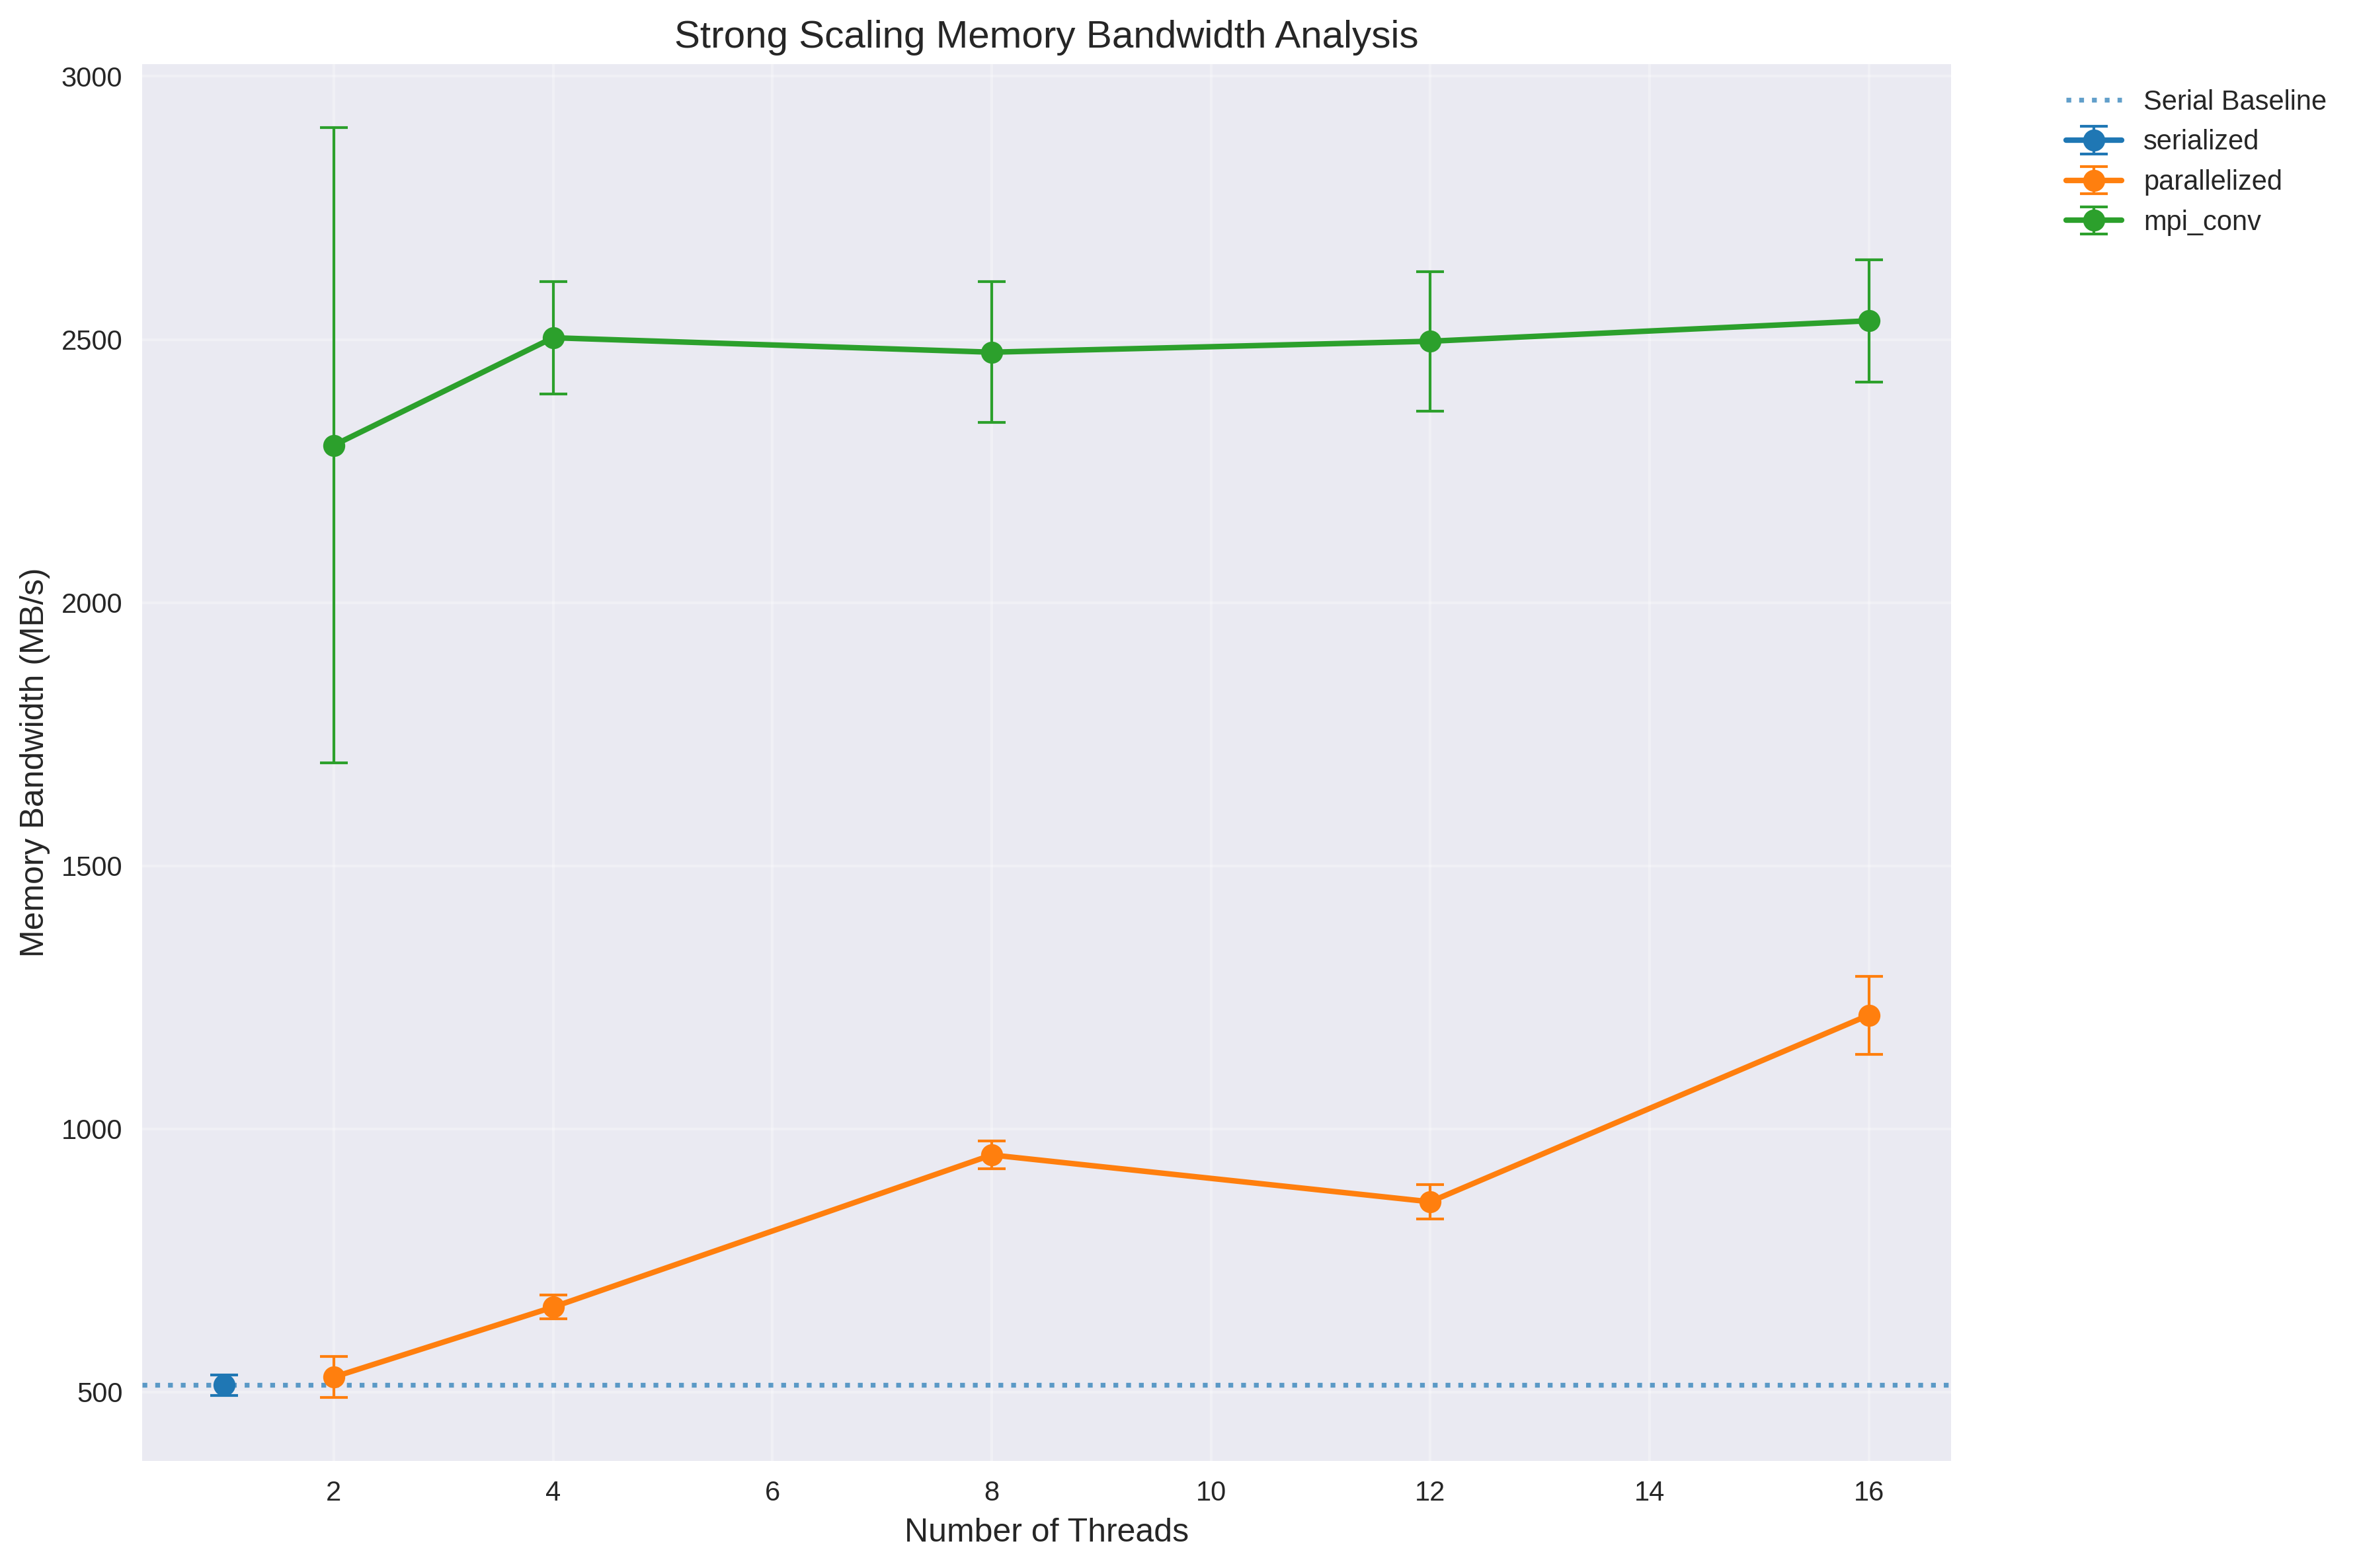
\includegraphics[width=0.7\linewidth]{figures/mem_bandwidth_vs_threads.png} \caption{Strong Mem. Bandwidth.}\label{fig:strong-scaling-mem-bw}\end{figure}
    \textbf{IPC (Fig.~\ref{fig:strong-scaling-ipc}):} mpi\_conv IPC dropped significantly; `parallelized` IPC increased with threads (efficient small work execution) but overall speedup remained poor.
\begin{figure}[H] \centering 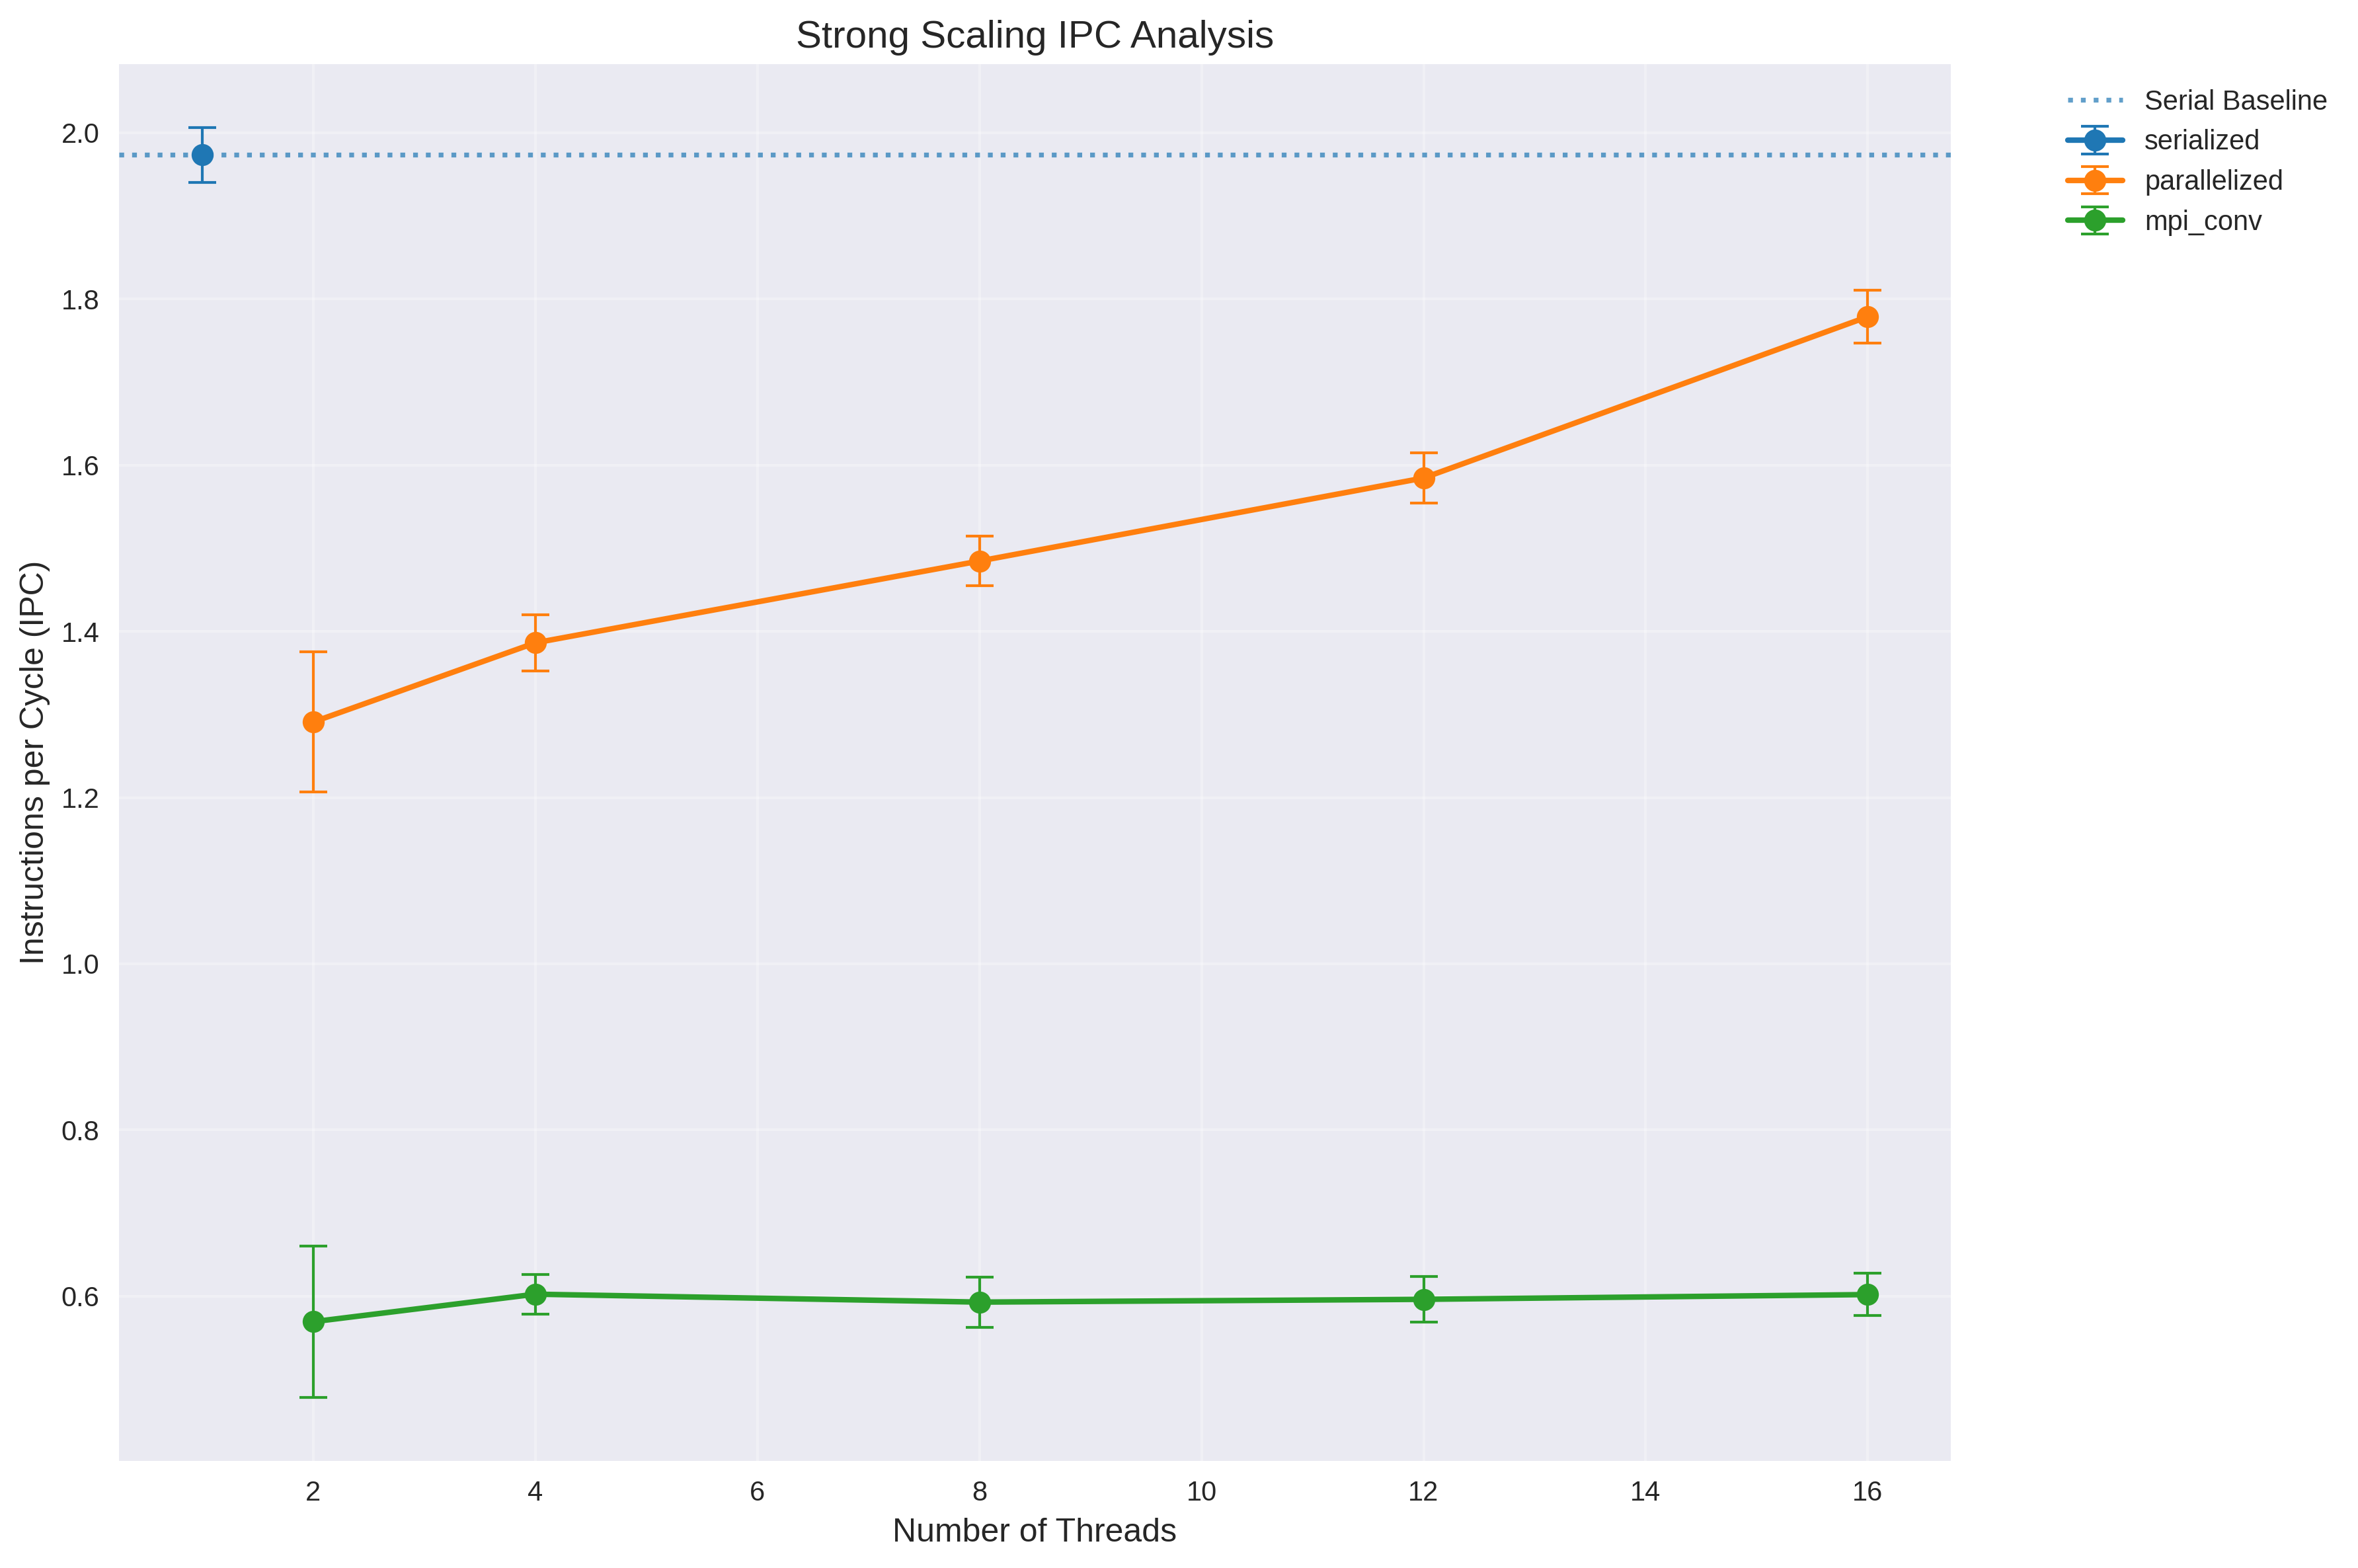
\includegraphics[width=0.7\linewidth]{figures/ipc_vs_threads.png} \caption{Strong IPC.}\label{fig:strong-scaling-ipc}\end{figure}
    \textbf{Execution Time:} mpi\_conv faster, stabilized early; `parallelized` slower.
    \textbf{Parallel Efficiency (Fig.~\ref{fig:strong-scaling-efficiency}):} mpi\_conv high initially then dropped; `parallelized` low throughout.
\begin{figure}[H] \centering 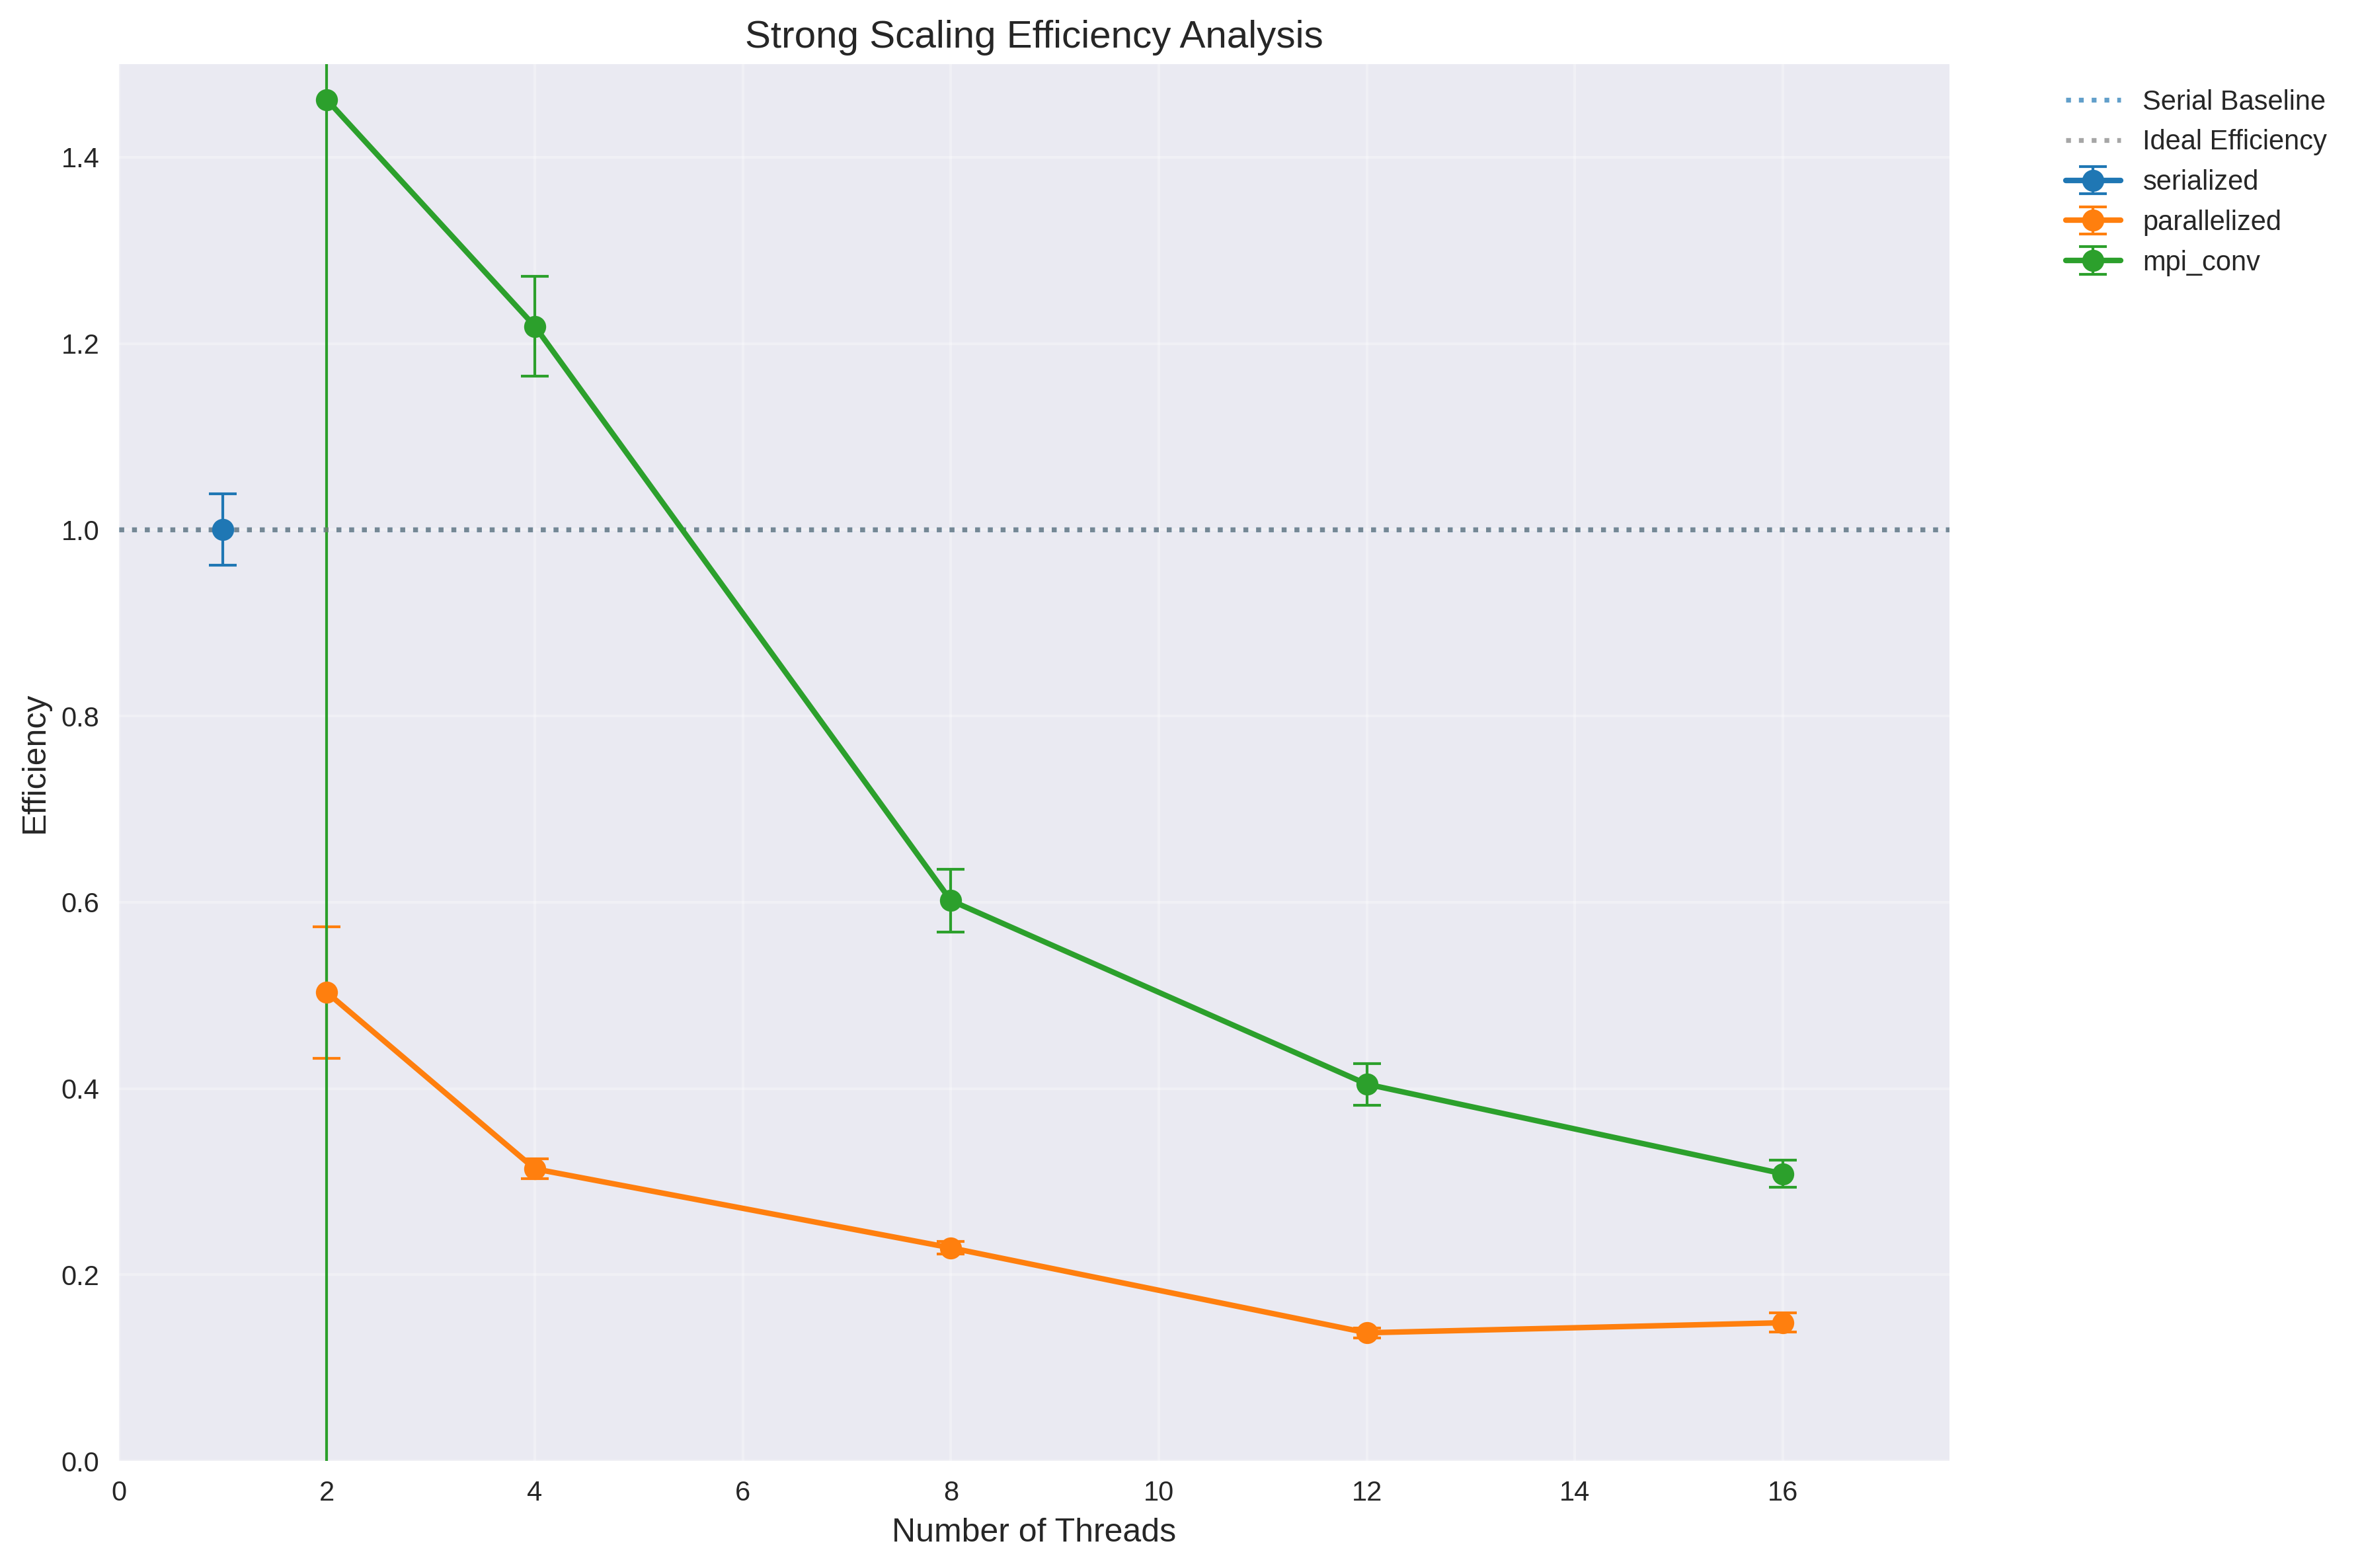
\includegraphics[width=0.7\linewidth]{figures/efficiency_vs_threads.png} \caption{Strong Efficiency \cite{Rajput2013}.}\label{fig:strong-scaling-efficiency}\end{figure}
    \textbf{L1 Cache Miss Rate (Fig.~\ref{fig:strong-scaling-l1-miss}):} mpi\_conv rate doubled; `parallelized` low/stable near serial \cite{Yoon2012}.
\begin{figure}[H] \centering 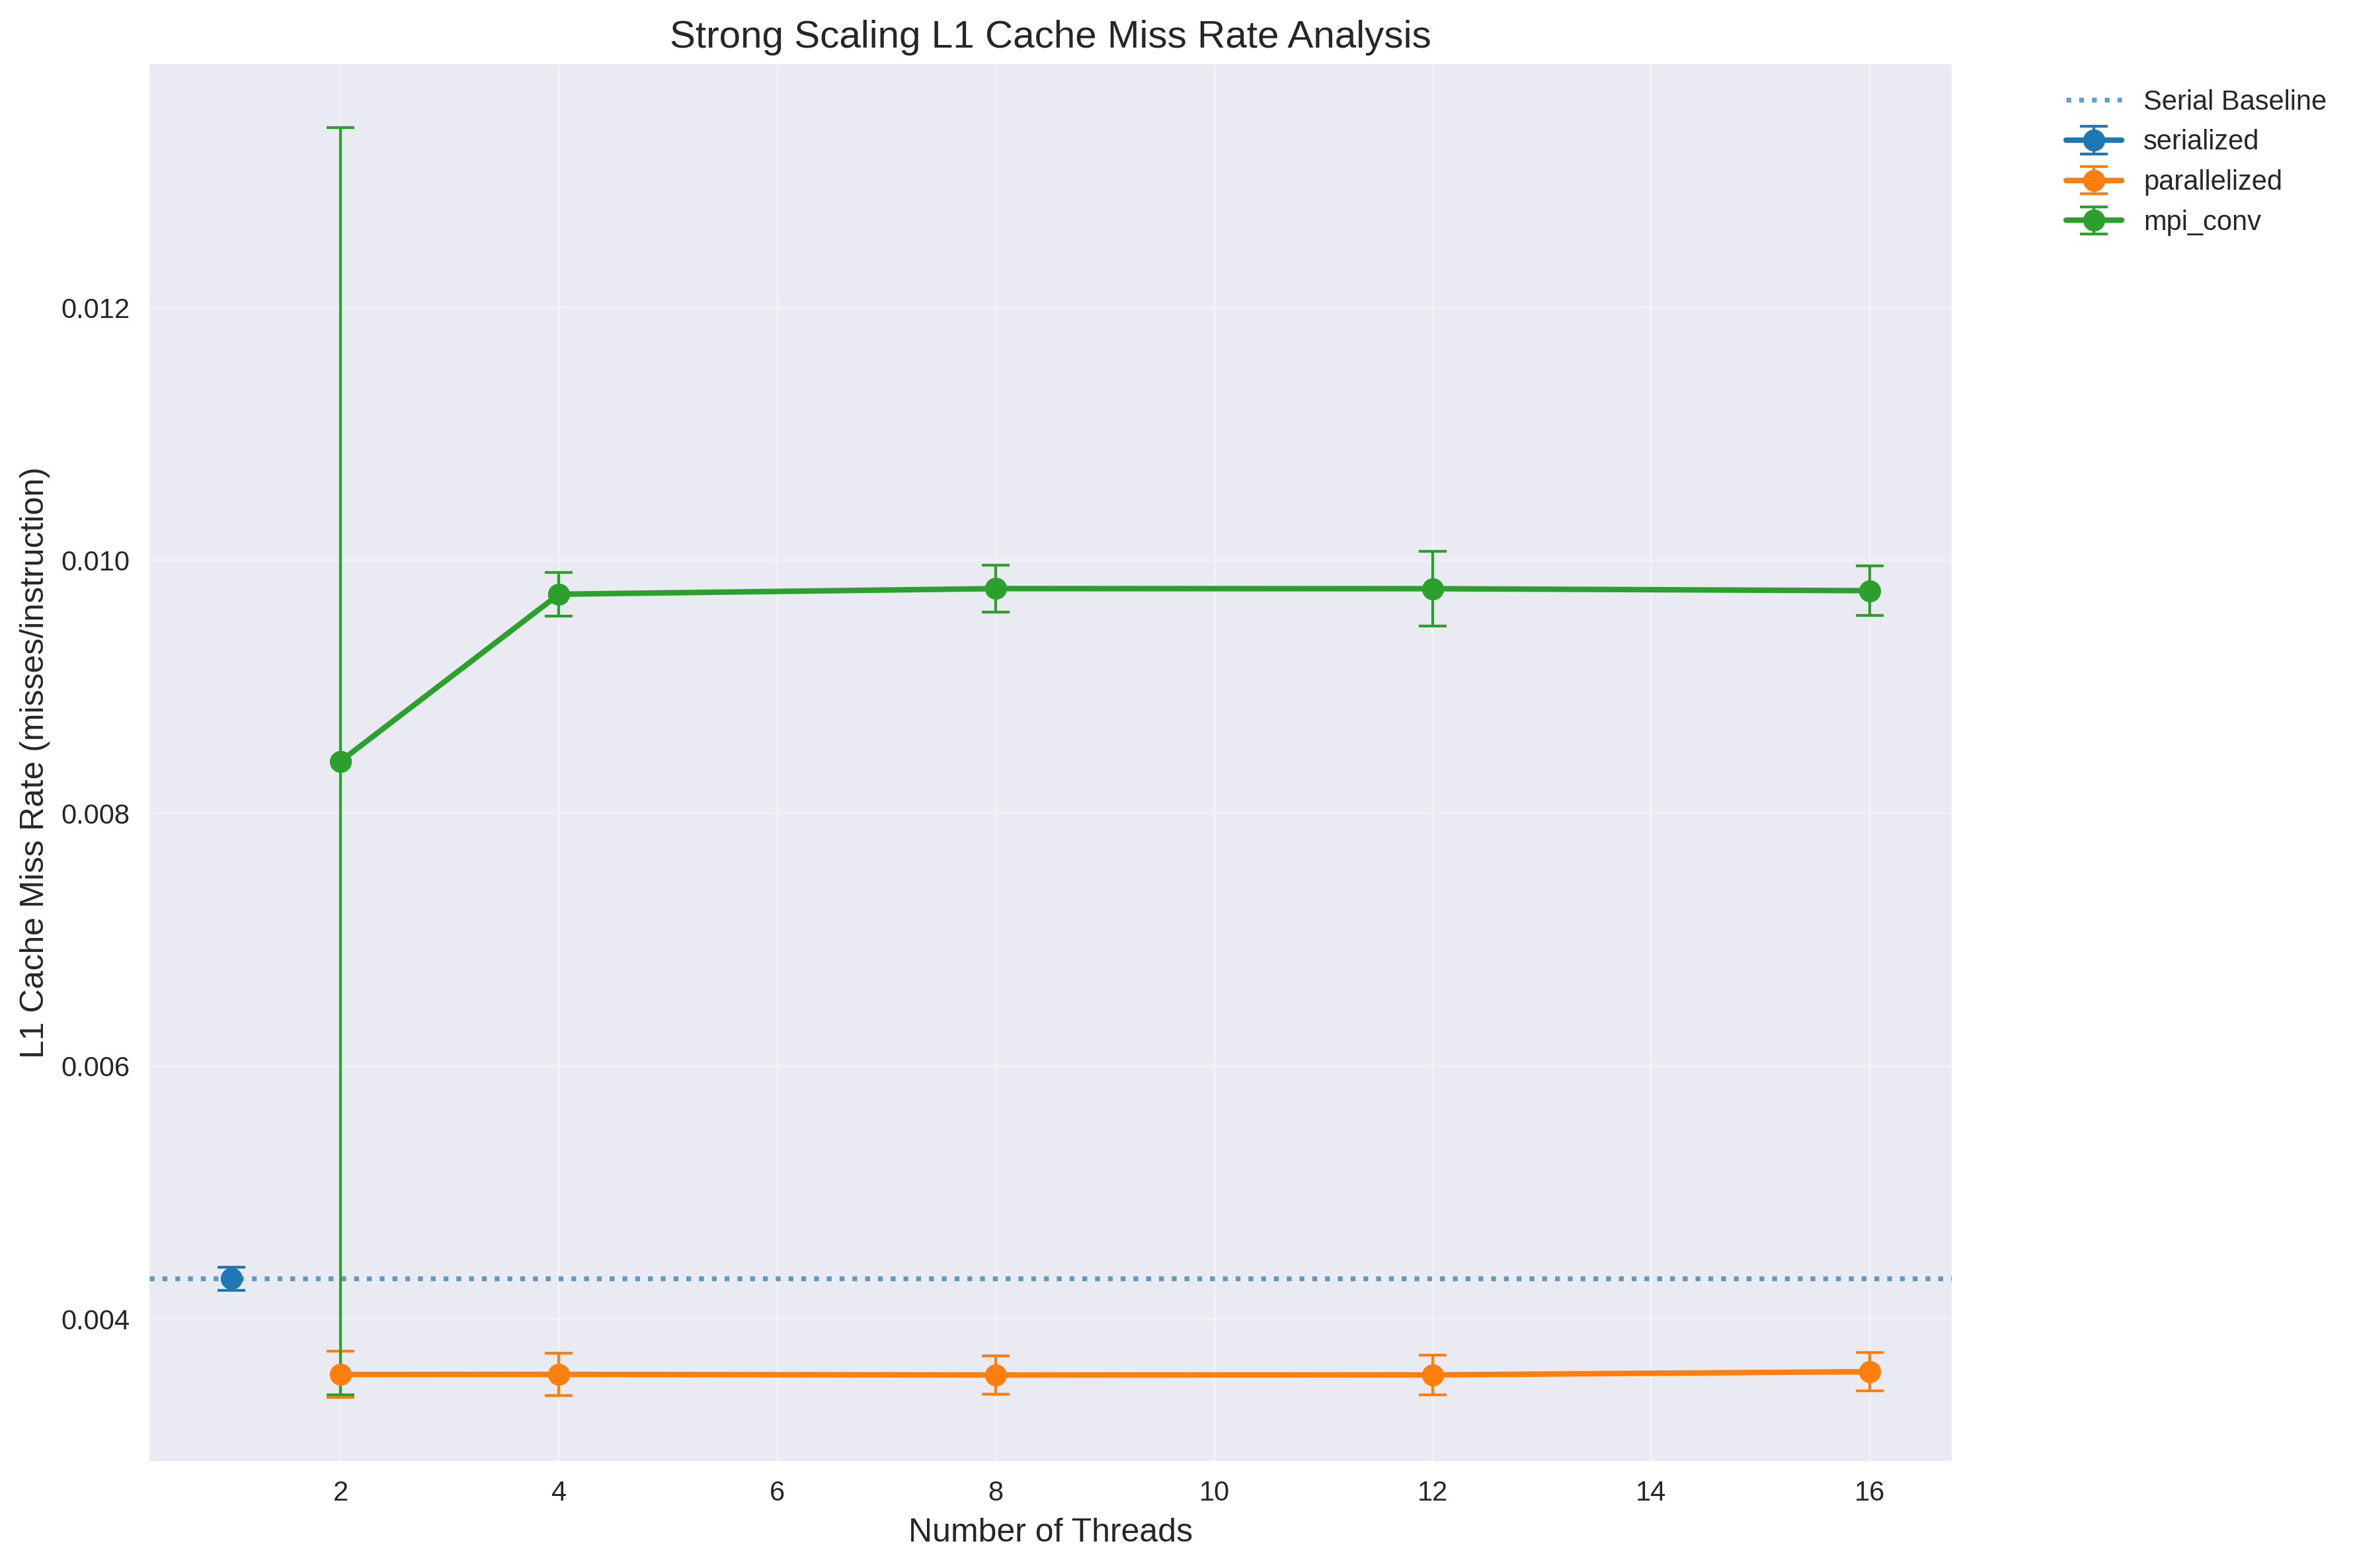
\includegraphics[width=0.7\linewidth]{figures/l1_miss_rate_vs_threads.png} \caption{Strong L1 Miss Rate.}\label{fig:strong-scaling-l1-miss}\end{figure}

\textbf{3. Summary of Strong Scaling Findings}
\begin{itemize}
    \item MPI-only mpi\_conv outperformed `parallelized` in strong scaling.
    \item mpi\_conv limited after 4 processes; `parallelized` struggled with hybrid overheads on the fixed problem size, despite good per-thread IPC and L1 cache behavior.
    \item Results highlight that optimal parallel strategy is highly dependent on scaling regime and problem size relative to core count.
\end{itemize}




% ====================================================================
% --- CONCLUSION AND FUTURE WORK ---
% ====================================================================
\section{Conclusion and Future Work}

This research demonstrated the acceleration of 2D convolution kernels on multi-core CPUs and GPUs using MPI, OpenMP, and CUDA.

The CUDA implementation on an NVIDIA RTX 3050 GPU achieved a significant speedup of approximately 11.7$\times$ over the sequential CPU version, highlighting the massive parallelism available on GPUs. Nsight Compute profiling revealed that the kernel was largely compute-bound with high L1/L2 cache hit rates, though opportunities exist for improving memory coalescing and reducing texture unit stalls.

For multi-core CPU parallelism, the hybrid OpenMP+MPI (`parallelized`) approach exhibited superior performance in weak scaling scenarios, achieving near-ideal scalability with constant execution time as problem size and core count increased proportionally. This indicates effective management of parallelism overheads and efficient use of shared memory resources \cite{Gawrych2023}. Conversely, in strong scaling experiments with a fixed problem size, the MPI-only (`mpi-conv`) version outperformed the hybrid model, particularly up to 4 processes, after which its benefits diminished due to Amdahl's Law limitations \cite{hager2021hpc} and increased MPI communication overheads. The hybrid model struggled in strong scaling due to the combined overheads of MPI and OpenMP becoming significant relative to the reduced work per thread. These contrasting results underscore that the optimal parallelization strategy is highly dependent on the scaling regime and the problem size-to-core ratio.

Future work:
Future work will focus on several architectural, tooling, and evaluation dimensions to further advance the performance and applicability of the proposed parallelization strategies.

On the GPU side, additional optimizations of memory access patterns—particularly improvements in memory coalescing and shared memory utilization—are expected to yield further performance gains. Investigating advanced CUDA features such as dynamic parallelism and asynchronous operations may also enhance pipeline efficiency, particularly for more complex or nested computational tasks.

For CPU-based parallelism, future efforts will involve evaluating alternative domain decomposition strategies and implementing more sophisticated hybrid load balancing mechanisms, particularly under strong scaling scenarios. Moreover, systematic experimentation across a broader set of CPU architectures—including variations in cache hierarchies, NUMA configurations, and interconnect topologies—will provide deeper insights into performance portability and architectural sensitivity.

The use of larger compute clusters will also be considered to assess the scalability limits of the current approach. In addition, the potential for heterogeneous acceleration will be explored further through the integration of alternative platforms such as FPGAs, which may offer energy-efficient acceleration for specific kernel classes.

In terms of development tools, comparative analysis involving other parallel programming models (e.g., OpenACC) and the use of auto-parallelizing compilers will be pursued to evaluate their efficacy and applicability relative to the current implementation.

Finally, the evaluation framework will be extended to include metrics such as power consumption, thermal behavior, and performance-per-watt. These considerations are essential for realistic deployment scenarios, particularly in energy-constrained or thermally sensitive environments.




% ====================================================================
% --- END OF MAIN PROPOSAL CONTENT ---
% ====================================================================


\section*{Acknowledgment} 
% Add acknowledgments
We thank Dr. Islam Tharwat Abdel Halim and Eng. Hassan Ahmed for their guidance.


% --- Bibliography Setup (Keep these lines) ---
\bibliographystyle{IEEEtran} 
\bibliography{references} % file is references.bib

\end{document}
% --- END OF FILE proposal.tex ---